\documentclass[english]{article}

\usepackage{babel}
\usepackage{graphicx}
\usepackage{times}
\usepackage{pifont}
\usepackage[margin=1in]{geometry}
\usepackage{eurosym}
\usepackage{fancyhdr}
\usepackage[hidelinks]{hyperref}
\usepackage{float}

\pagestyle{fancy}
\fancyhf{}


%HEADER
%**************************************************************************************
\pagestyle{fancy}
\fancyhf{}
%**************************************************************************************
\lhead{Amplitude modulation}		 	 
\rhead{Laboratory Work in Telecommunications} 
\lfoot{EFA12SF}
\cfoot{\thepage}
\rfoot{Dmitry Boronin\\ Nikolay Arsenov\\ Alexey Tukalo}
%**************************************************************************************

\date{}
\setlength\parindent{0pt}

\begin{document}

\title{\vspace{2in}Amplitude modulation\\
\small for Laboratory Work in Telecommunications\\
\vspace{0.5in}
\includegraphics{savonia.jpg}}

\nopagebreak
\maketitle


\vspace{3in}

\author{
\begin{flushright}
Dmitry Boronin, Nikolay Arsenov, Alexey Tukalo,\\
EFA12SF,\\
Information Technology,\\
Savonia University of Applied Sciences
\end{flushright}
}

\date{\today}
\thispagestyle{empty}

\newpage
\setcounter{page}{1}
\setcounter{tocdepth}{2}
\tableofcontents

\newpage

%MAIN CONTENT ******************************************************************************************************************
\section{Introduction}
In the modulation process, the baseband voice, video, or digital signal modifies
another, higher-frequency signal called the carrier, which is usually a sine wave.
A sine wave carrier can be modified by the intelligence signal through amplitude modulation, frequency modulation, or phase modulation. The focus of this lab work is amplitude modulation (AM).
\subsection{Concept}
As the name suggests, in AM, the information signal varies the amplitude of the carrier
sine wave. The instantaneous value of the carrier amplitude changes in accordance with
the amplitude and frequency variations of the modulating signal. The carrier
frequency remains constant during the modulation process, but its amplitude varies in
accordance with the modulating signal. An increase in the amplitude of the modulating
signal causes the amplitude of the carrier to increase. Both the positive and the negative
peaks of the carrier wave vary with the modulating signal. An increase or a decrease in
the amplitude of the modulating signal causes a corresponding increase or decrease in both
the positive and the negative peaks of the carrier amplitude.\\\\
An imaginary line connecting the positive peaks and negative peaks of the carrier
waveform (the dashed line in Fig. 3-1) gives the exact shape of the modulating
information signal. This imaginary line on the carrier waveform is known as the
envelope.\\\\
Using trigonometric functions, we can express the sine wave carrier with the simple
expression
$$
\upsilon_c=V_c \sin(2\pi f_ct)
$$
In this expression, $\upsilon_c$ represents the instantaneous value of the carrier sine wave voltage
at some specific time in the cycle; $V_c$ represents the peak value of the constant unmodulated carrier sine wave as measured between zero and the maximum amplitude of either
the positive-going or the negative-going alternations; $f_c$ is the frequency of the
carrier sine wave; and t is a particular point in time during the carrier cycle.\\\\
A sine wave modulating signal can be expressed with a similar formula
$$
\upsilon_m=V_m \sin(2 \pi f_m t)
$$
where $\upsilon_m$ = instantaneous value of information signal,
	$V_m$	  = peak amplitude of information signal,
	$f_m$ = frequency of modulating signal.
\subsection{History}
Although AM was used in a few crude experiments in multiplex telegraph and telephone transmission in the late 1800s, the practical development of amplitude modulation is synonymous with the development between 1900 and 1920 of "radiotelephone" transmission, that is, the effort to send sound (audio) by radio waves. The first radio transmitters, called spark gap transmitters, transmitted information by wireless telegraphy, using different length pulses of carrier wave to spell out text messages in Morse code. They couldn't transmit audio because the carrier consisted of strings of damped waves, pulses of radio waves that declined to zero, that sounded like a buzz in receivers. In effect they were already amplitude modulated.

\section{Materials}
During the laboratory work we used:
\begin{itemize}
\item Oscilloscope
\item Spectrum Analyser  
\item Different cables
\item Amplitude Modulation Transmitter Kit 
\item Amplitude Modulation Receiver Kit 
\begin{figure}[H]
\centerline{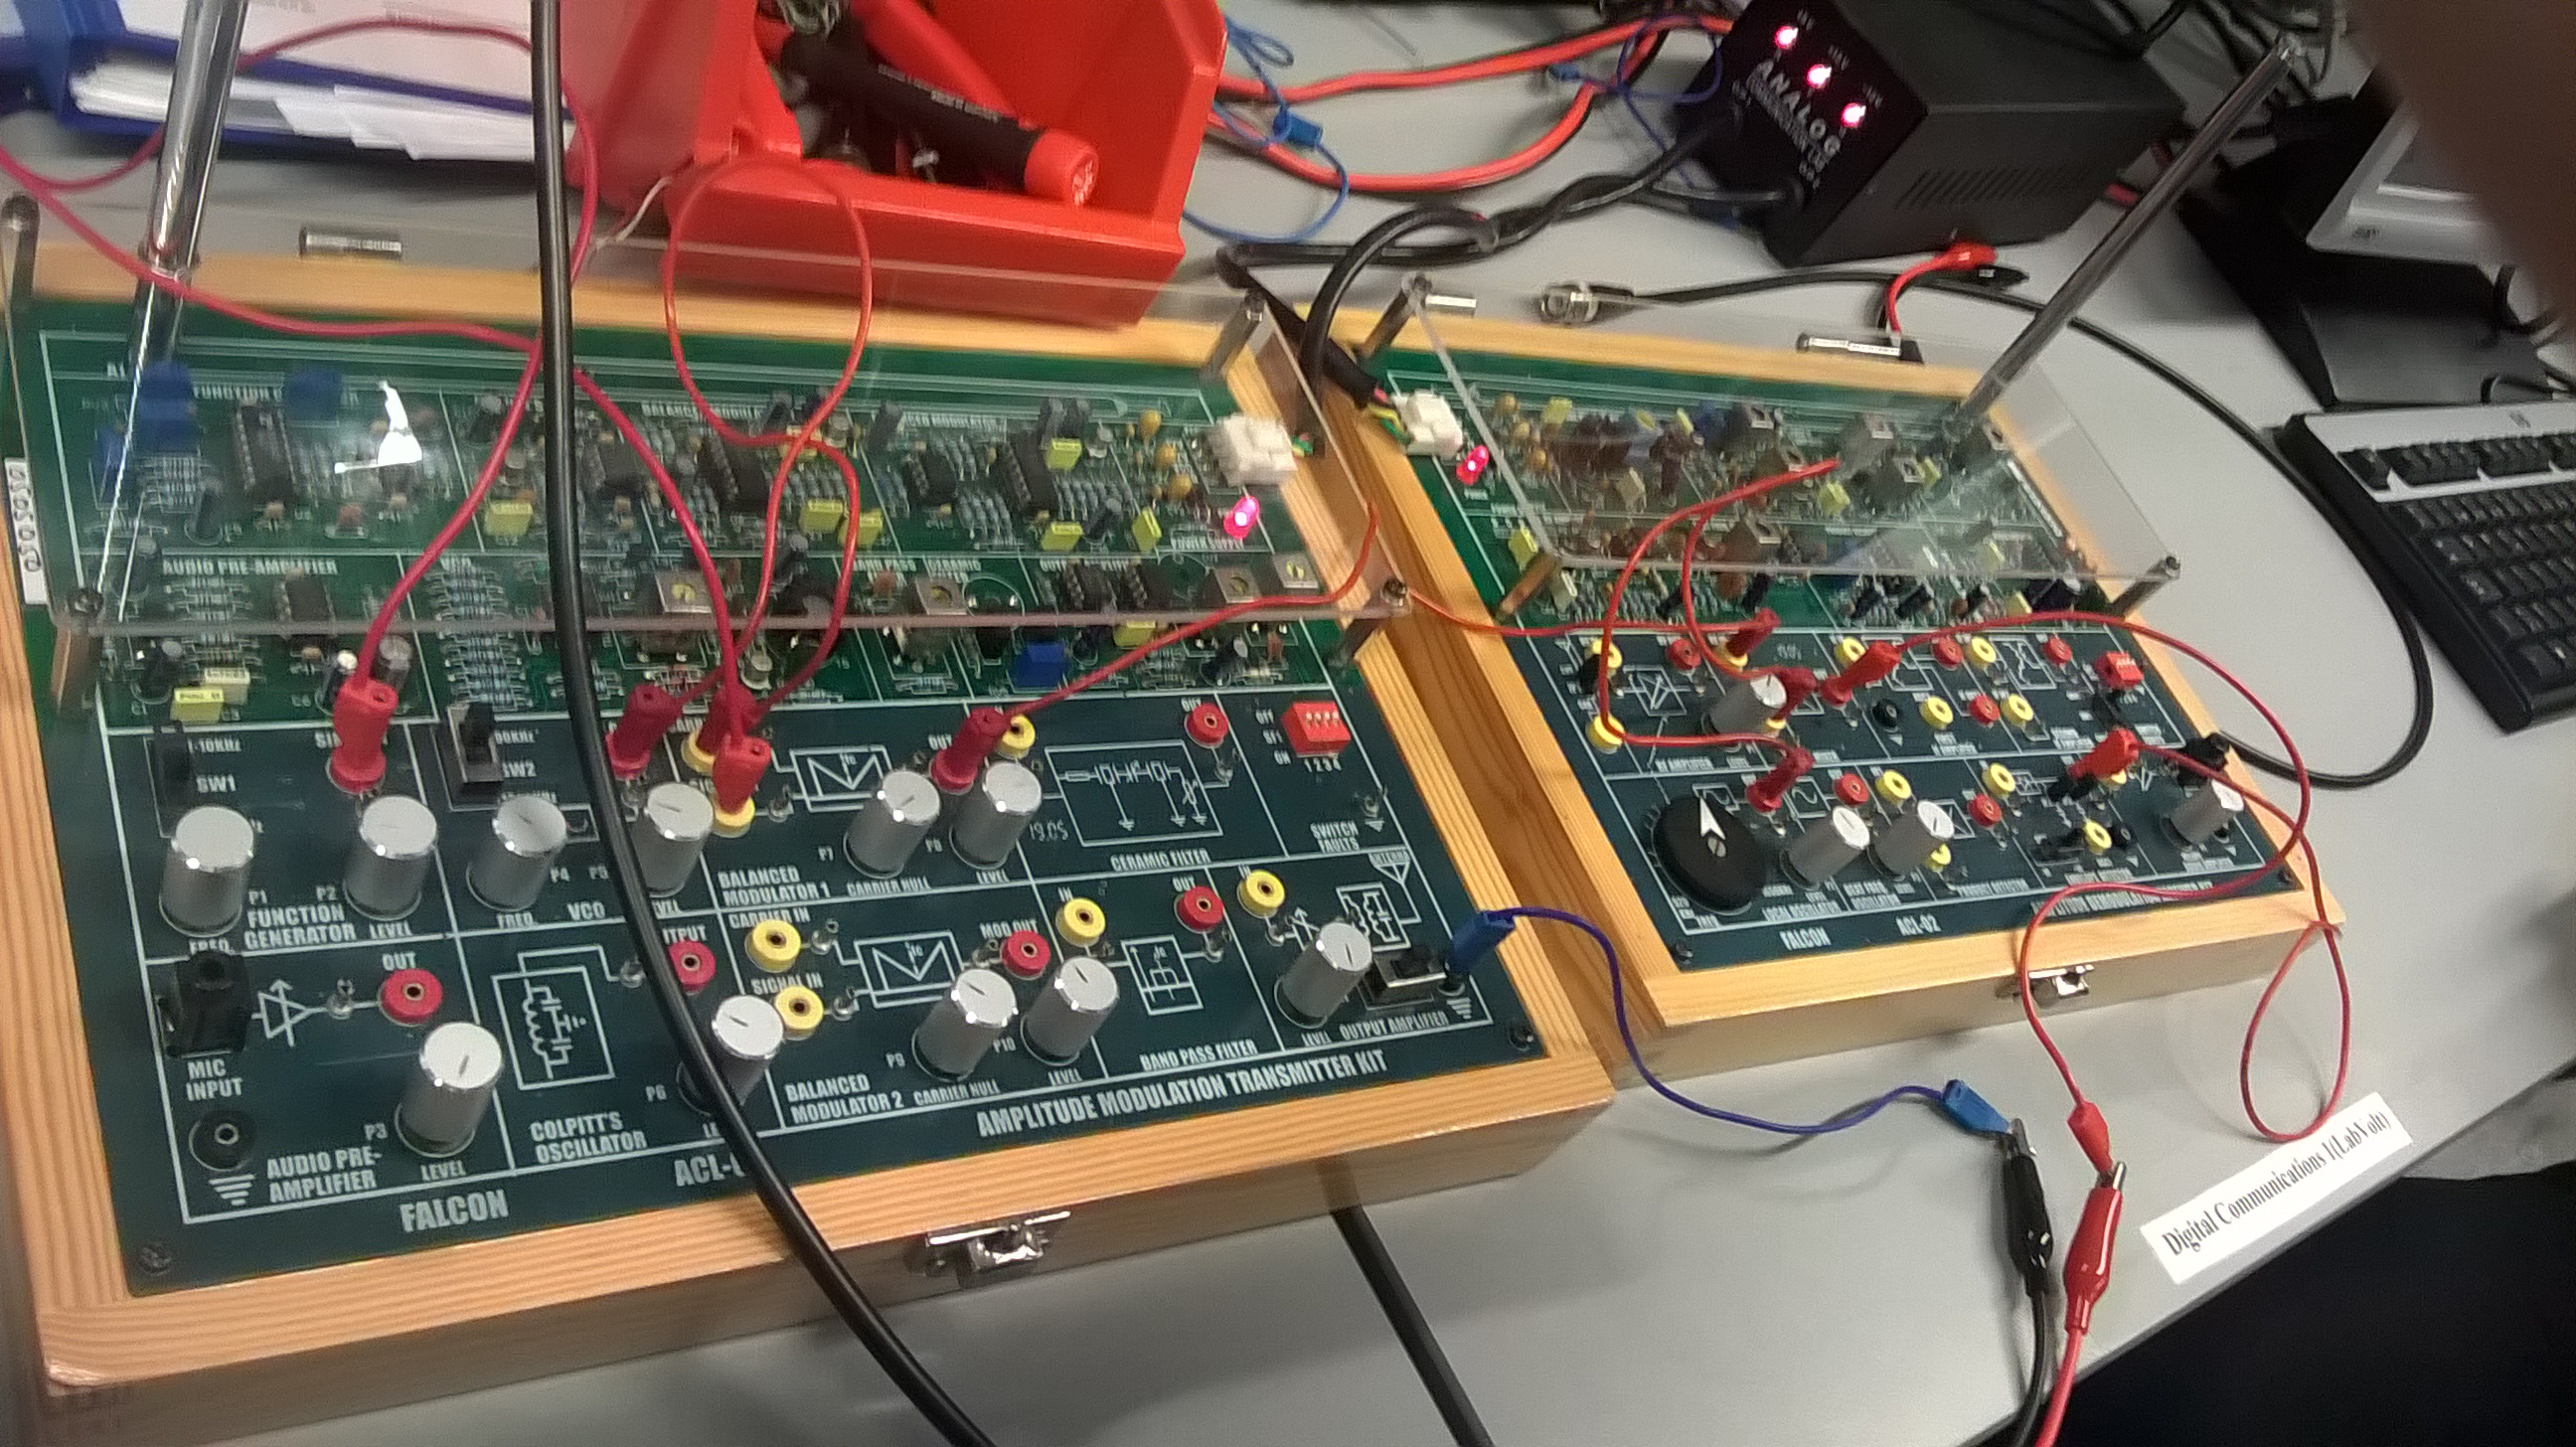
\includegraphics[scale=0.2]{AM/10Connection}}
\caption{Amplitude Modulation Transmitter and Receiver Kits with our connection}
\end{figure}
\end{itemize}


\section{Process of work}
\subsection{Modulation}
\subsubsection{Process of measurement}
\paragraph{At the first step} we have turn on a function generator on our Amplitude Modulation Transmitter Kit and set it on sin-wave mode with 1kHz frequency(figure 2).
\begin{figure}[H]
\centerline{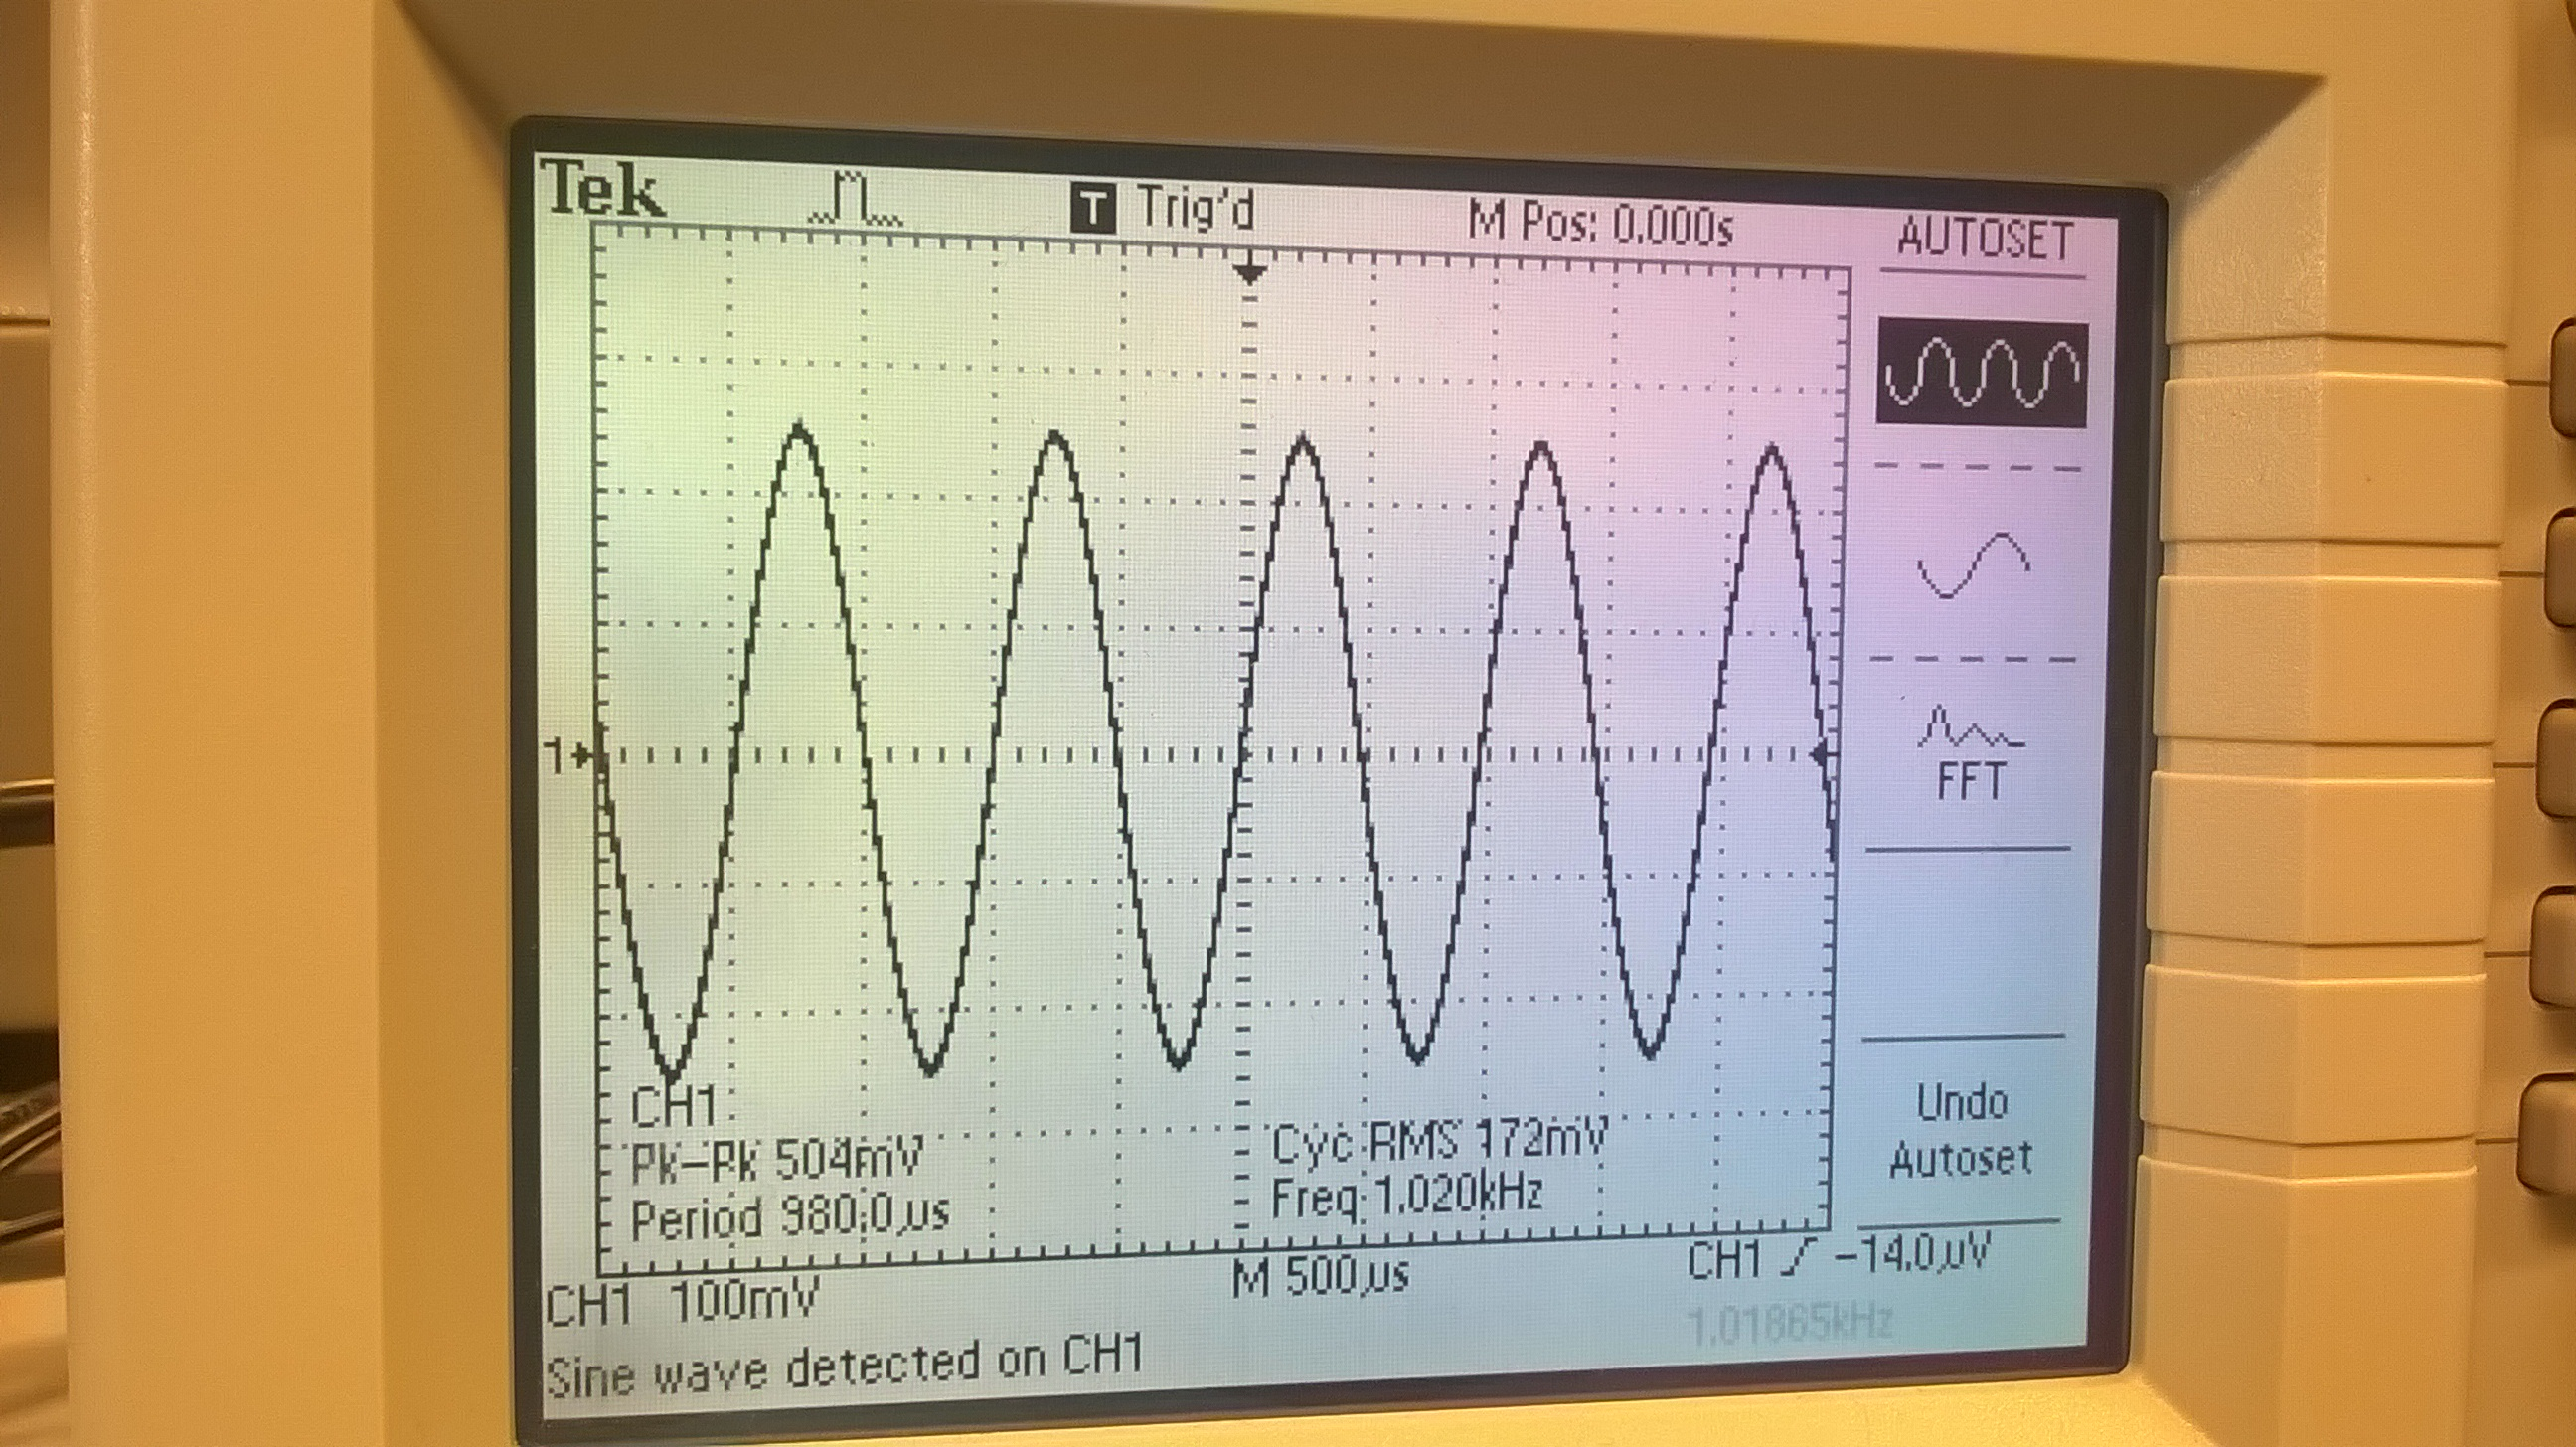
\includegraphics[scale=0.1]{AM/1AM_In}}
\caption{Oscilloscope output for the function generator}
\end{figure}
We also have measured the FFT of the signal on the oscilloscope(figure 3). The first big peak is representation of our main frequency.
\begin{figure}[H]
\centerline{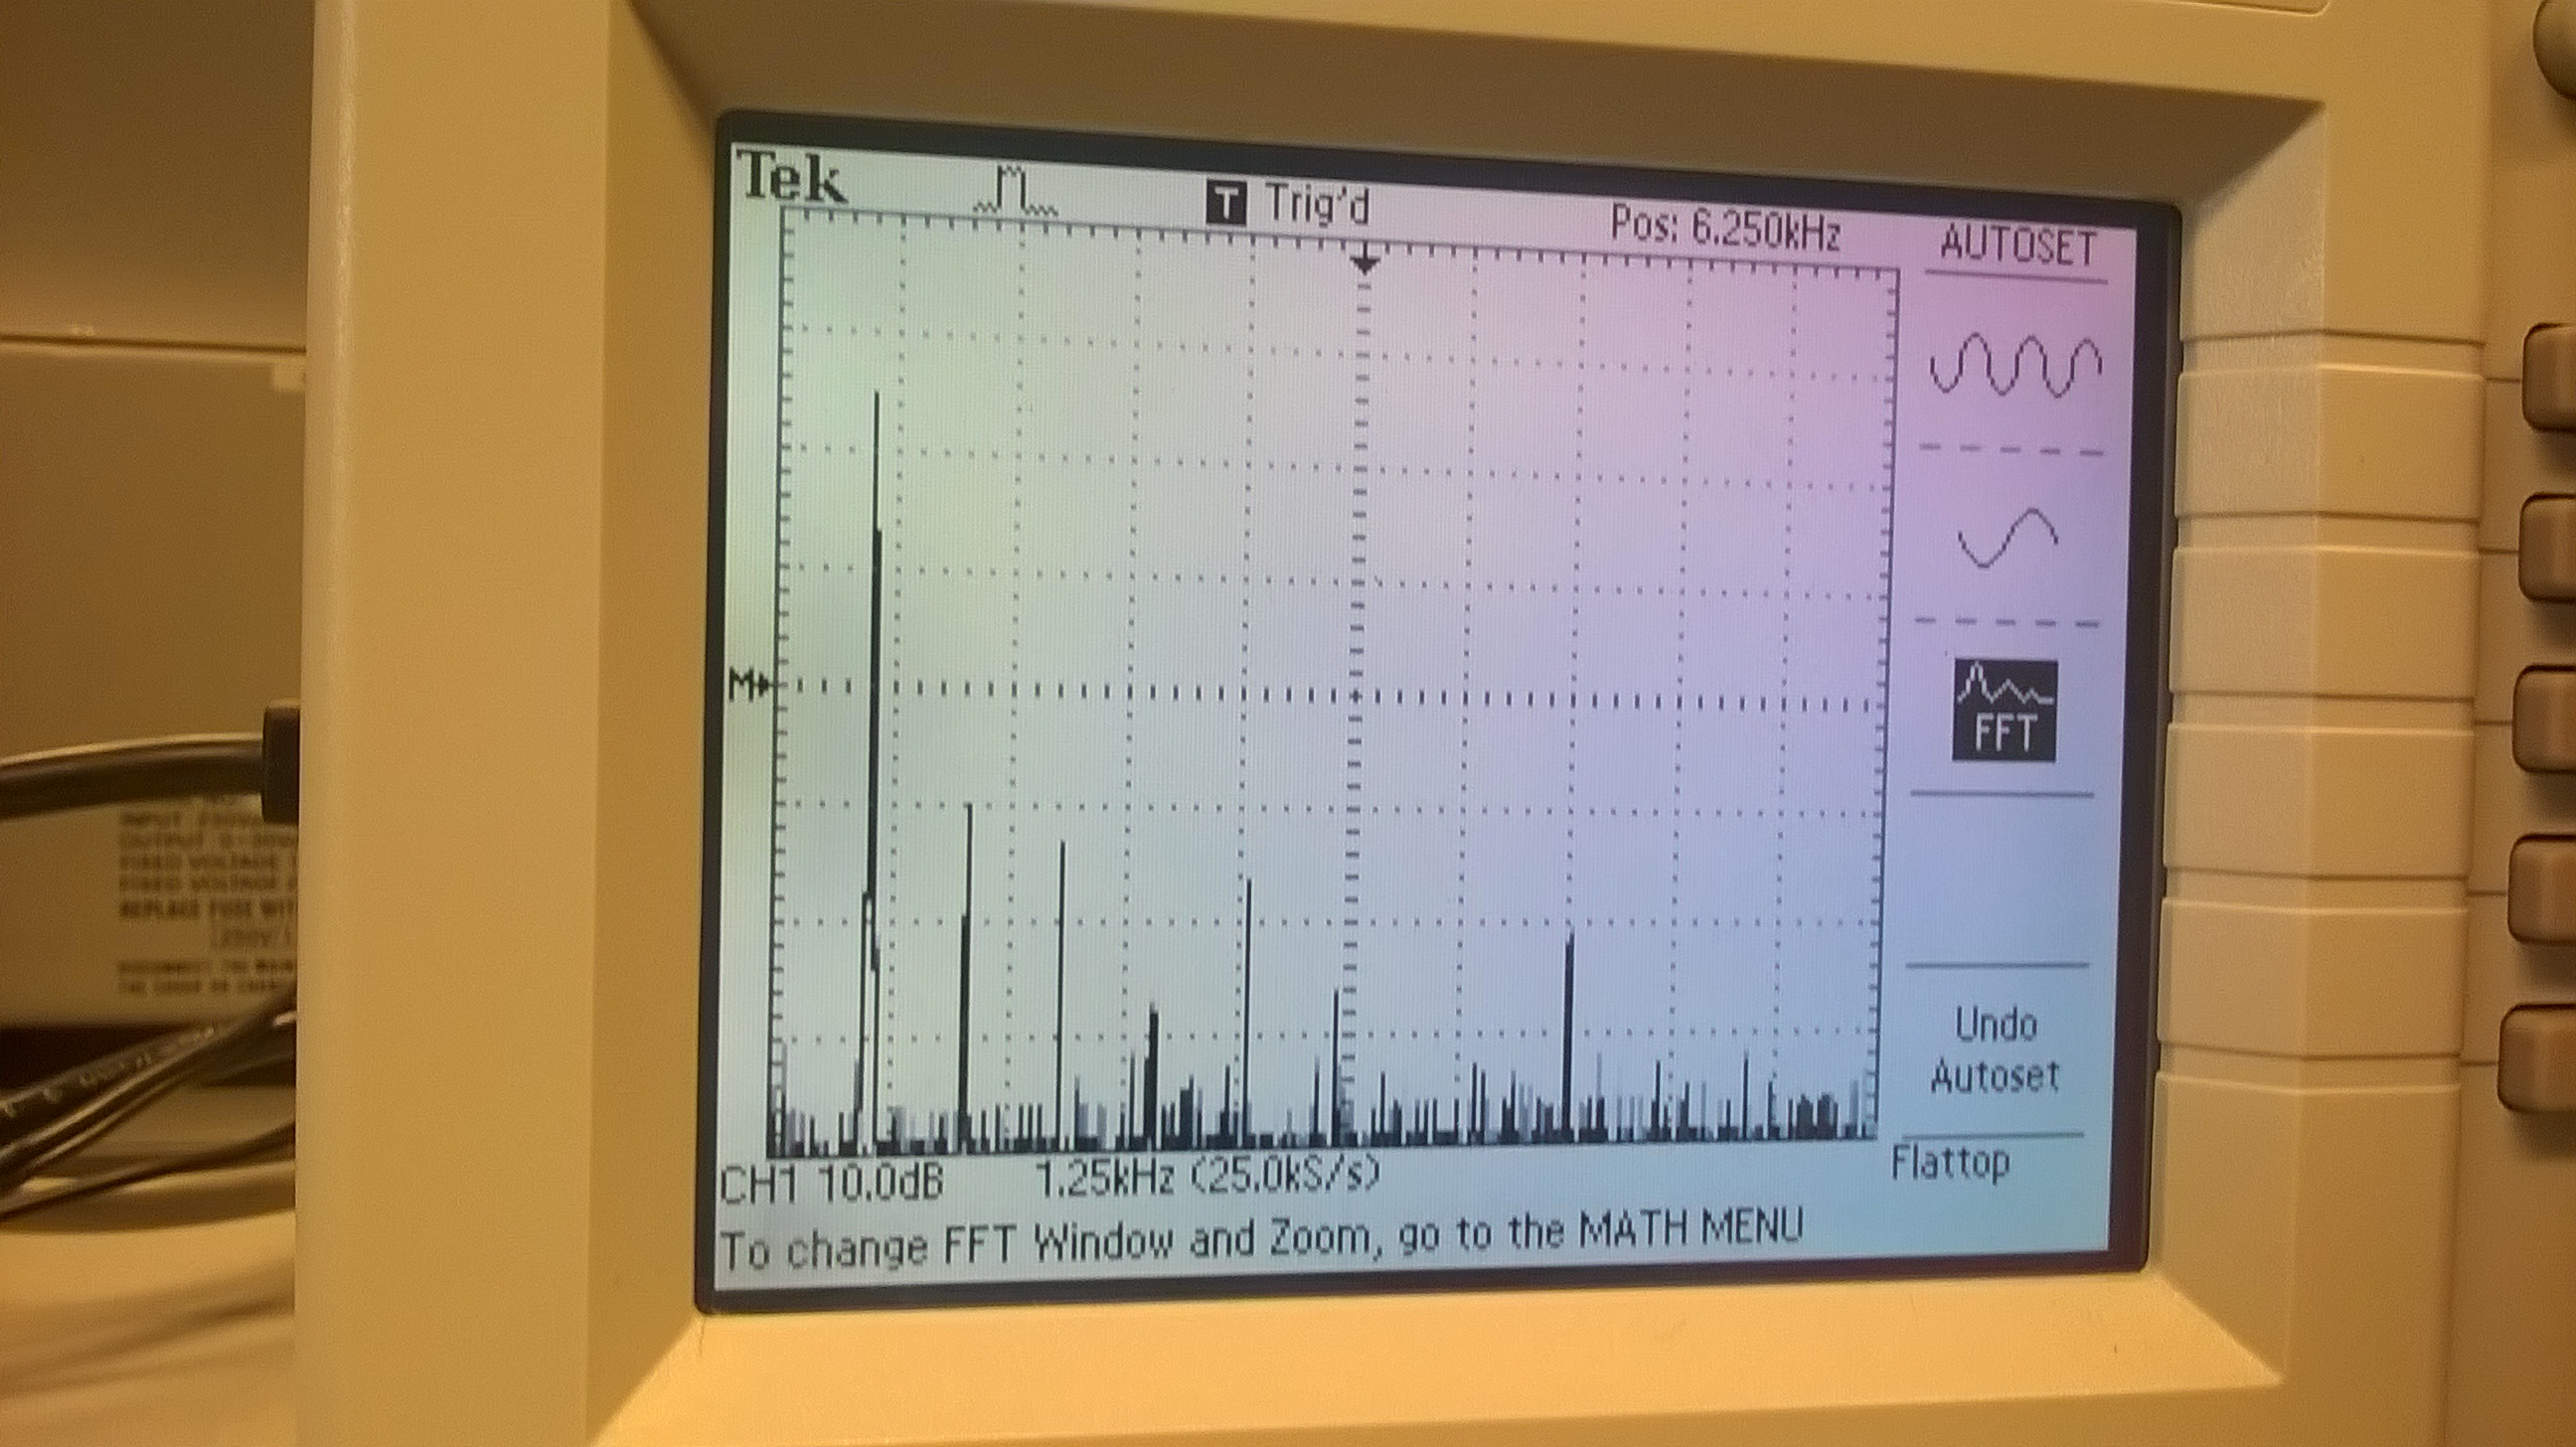
\includegraphics[scale=0.1]{AM/2IN_FFT}}
\caption{FFT of 1kHz signal}
\end{figure}
\paragraph{At the second} we set the signal of local oscillator, the frequency is 1.5MHz. The signal and the FFT representation of the signal is shown on the pictures 4 and 5.
\begin{figure}[H]
\centerline{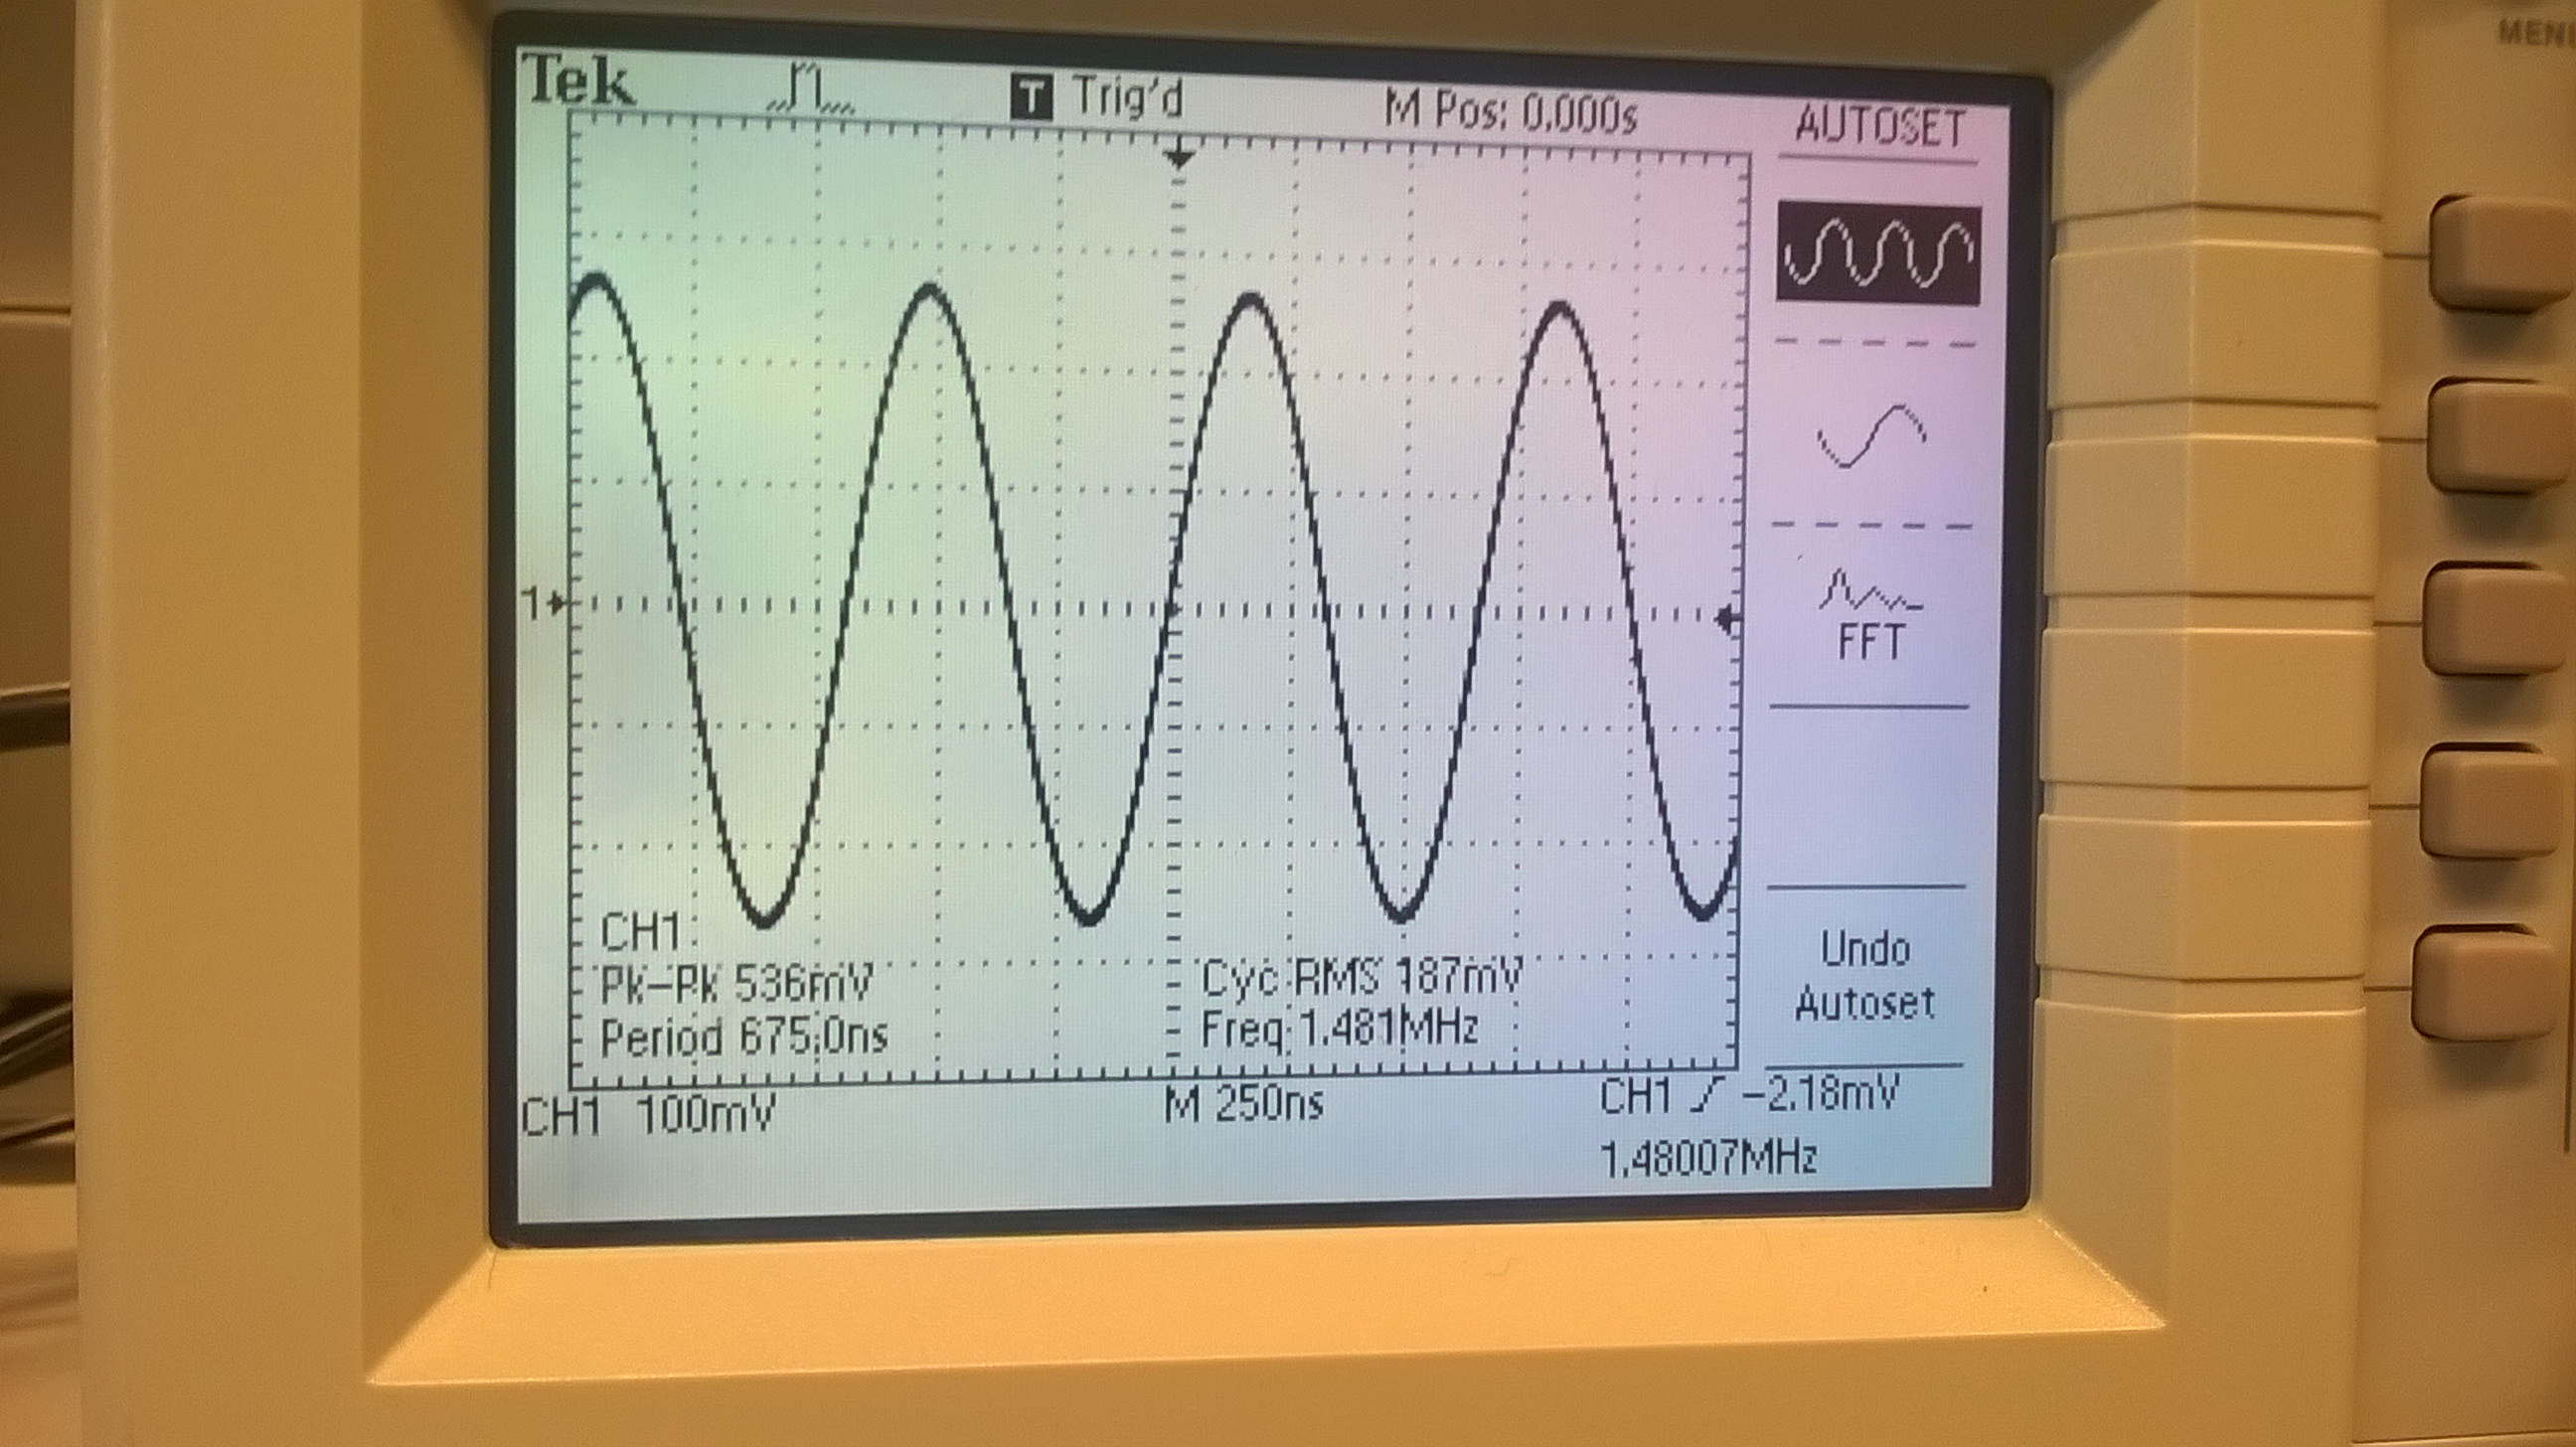
\includegraphics[scale=0.1]{AM/6LocalOscilator}}
\caption{The local oscillator signal}
\end{figure}
The local oscillator's signal also has sine form.
\begin{figure}[H]
\centerline{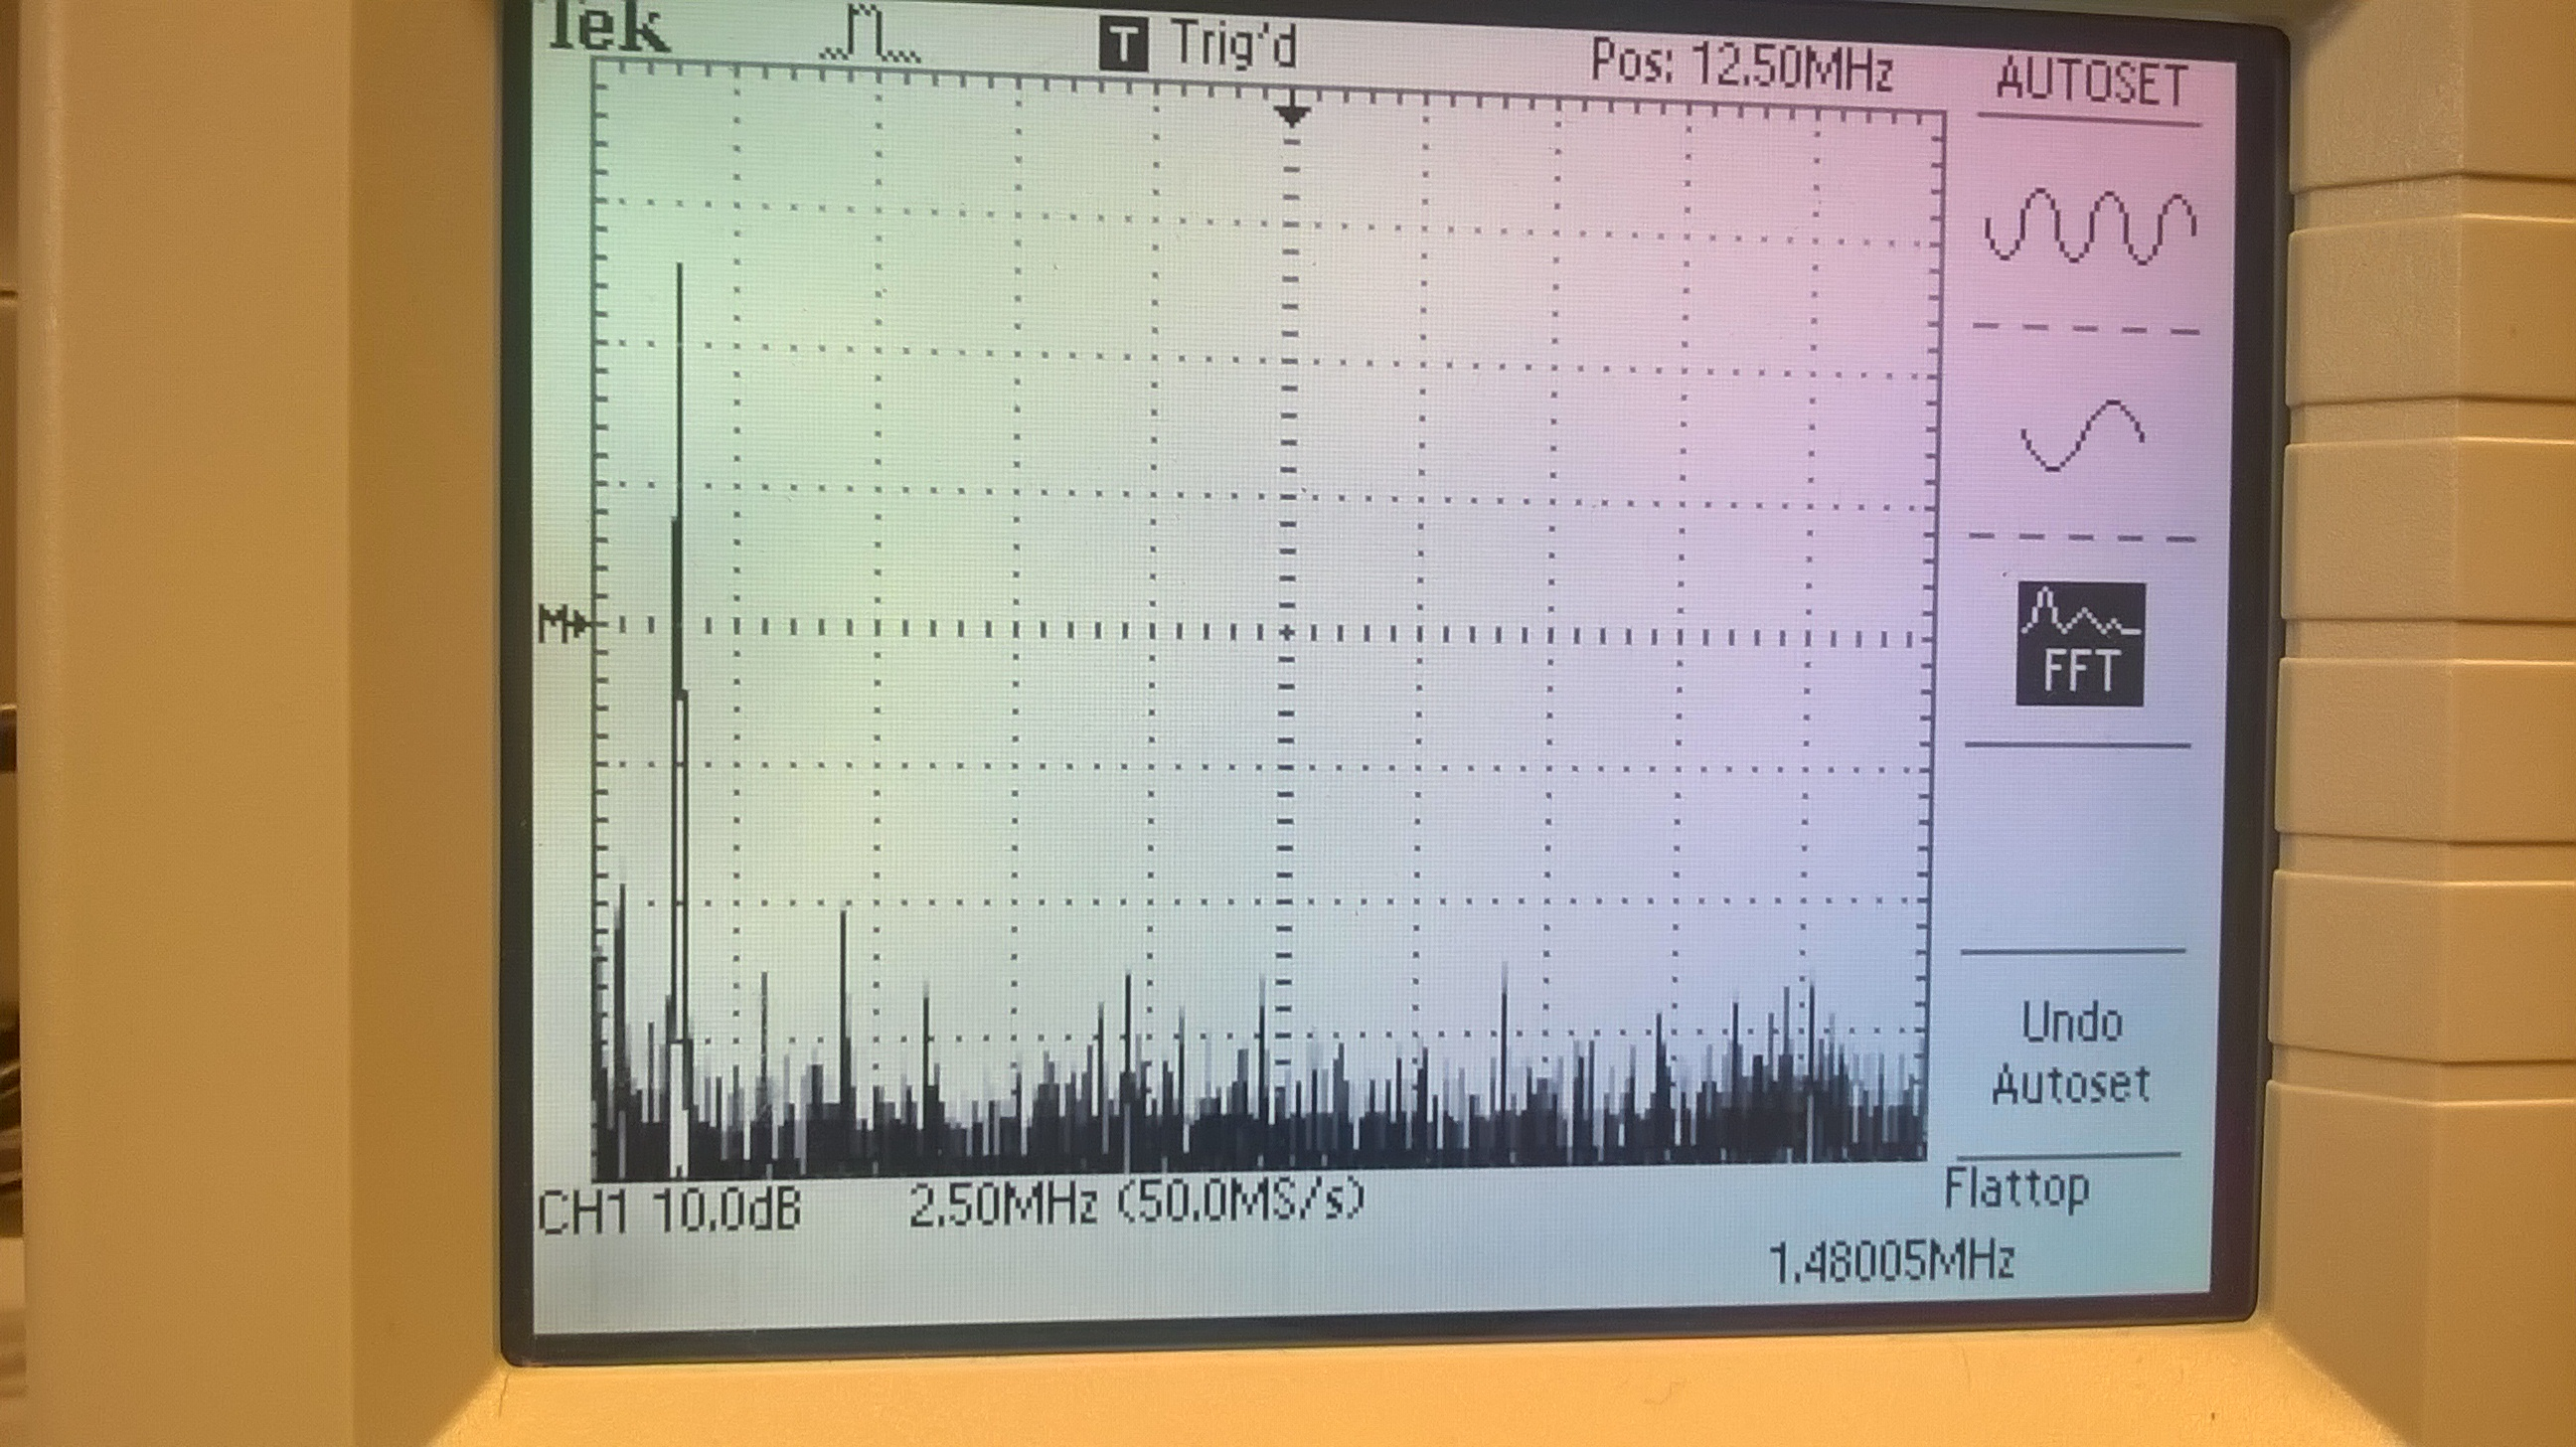
\includegraphics[scale=0.1]{AM/7FFTlocal}}
\caption{The FFT of local oscillator signal}
\end{figure}
\paragraph{After that} we can put the signal to the inputs of the Balanced Modulator and it will produce the modulated signal on the output.
\begin{figure}[H]
\centerline{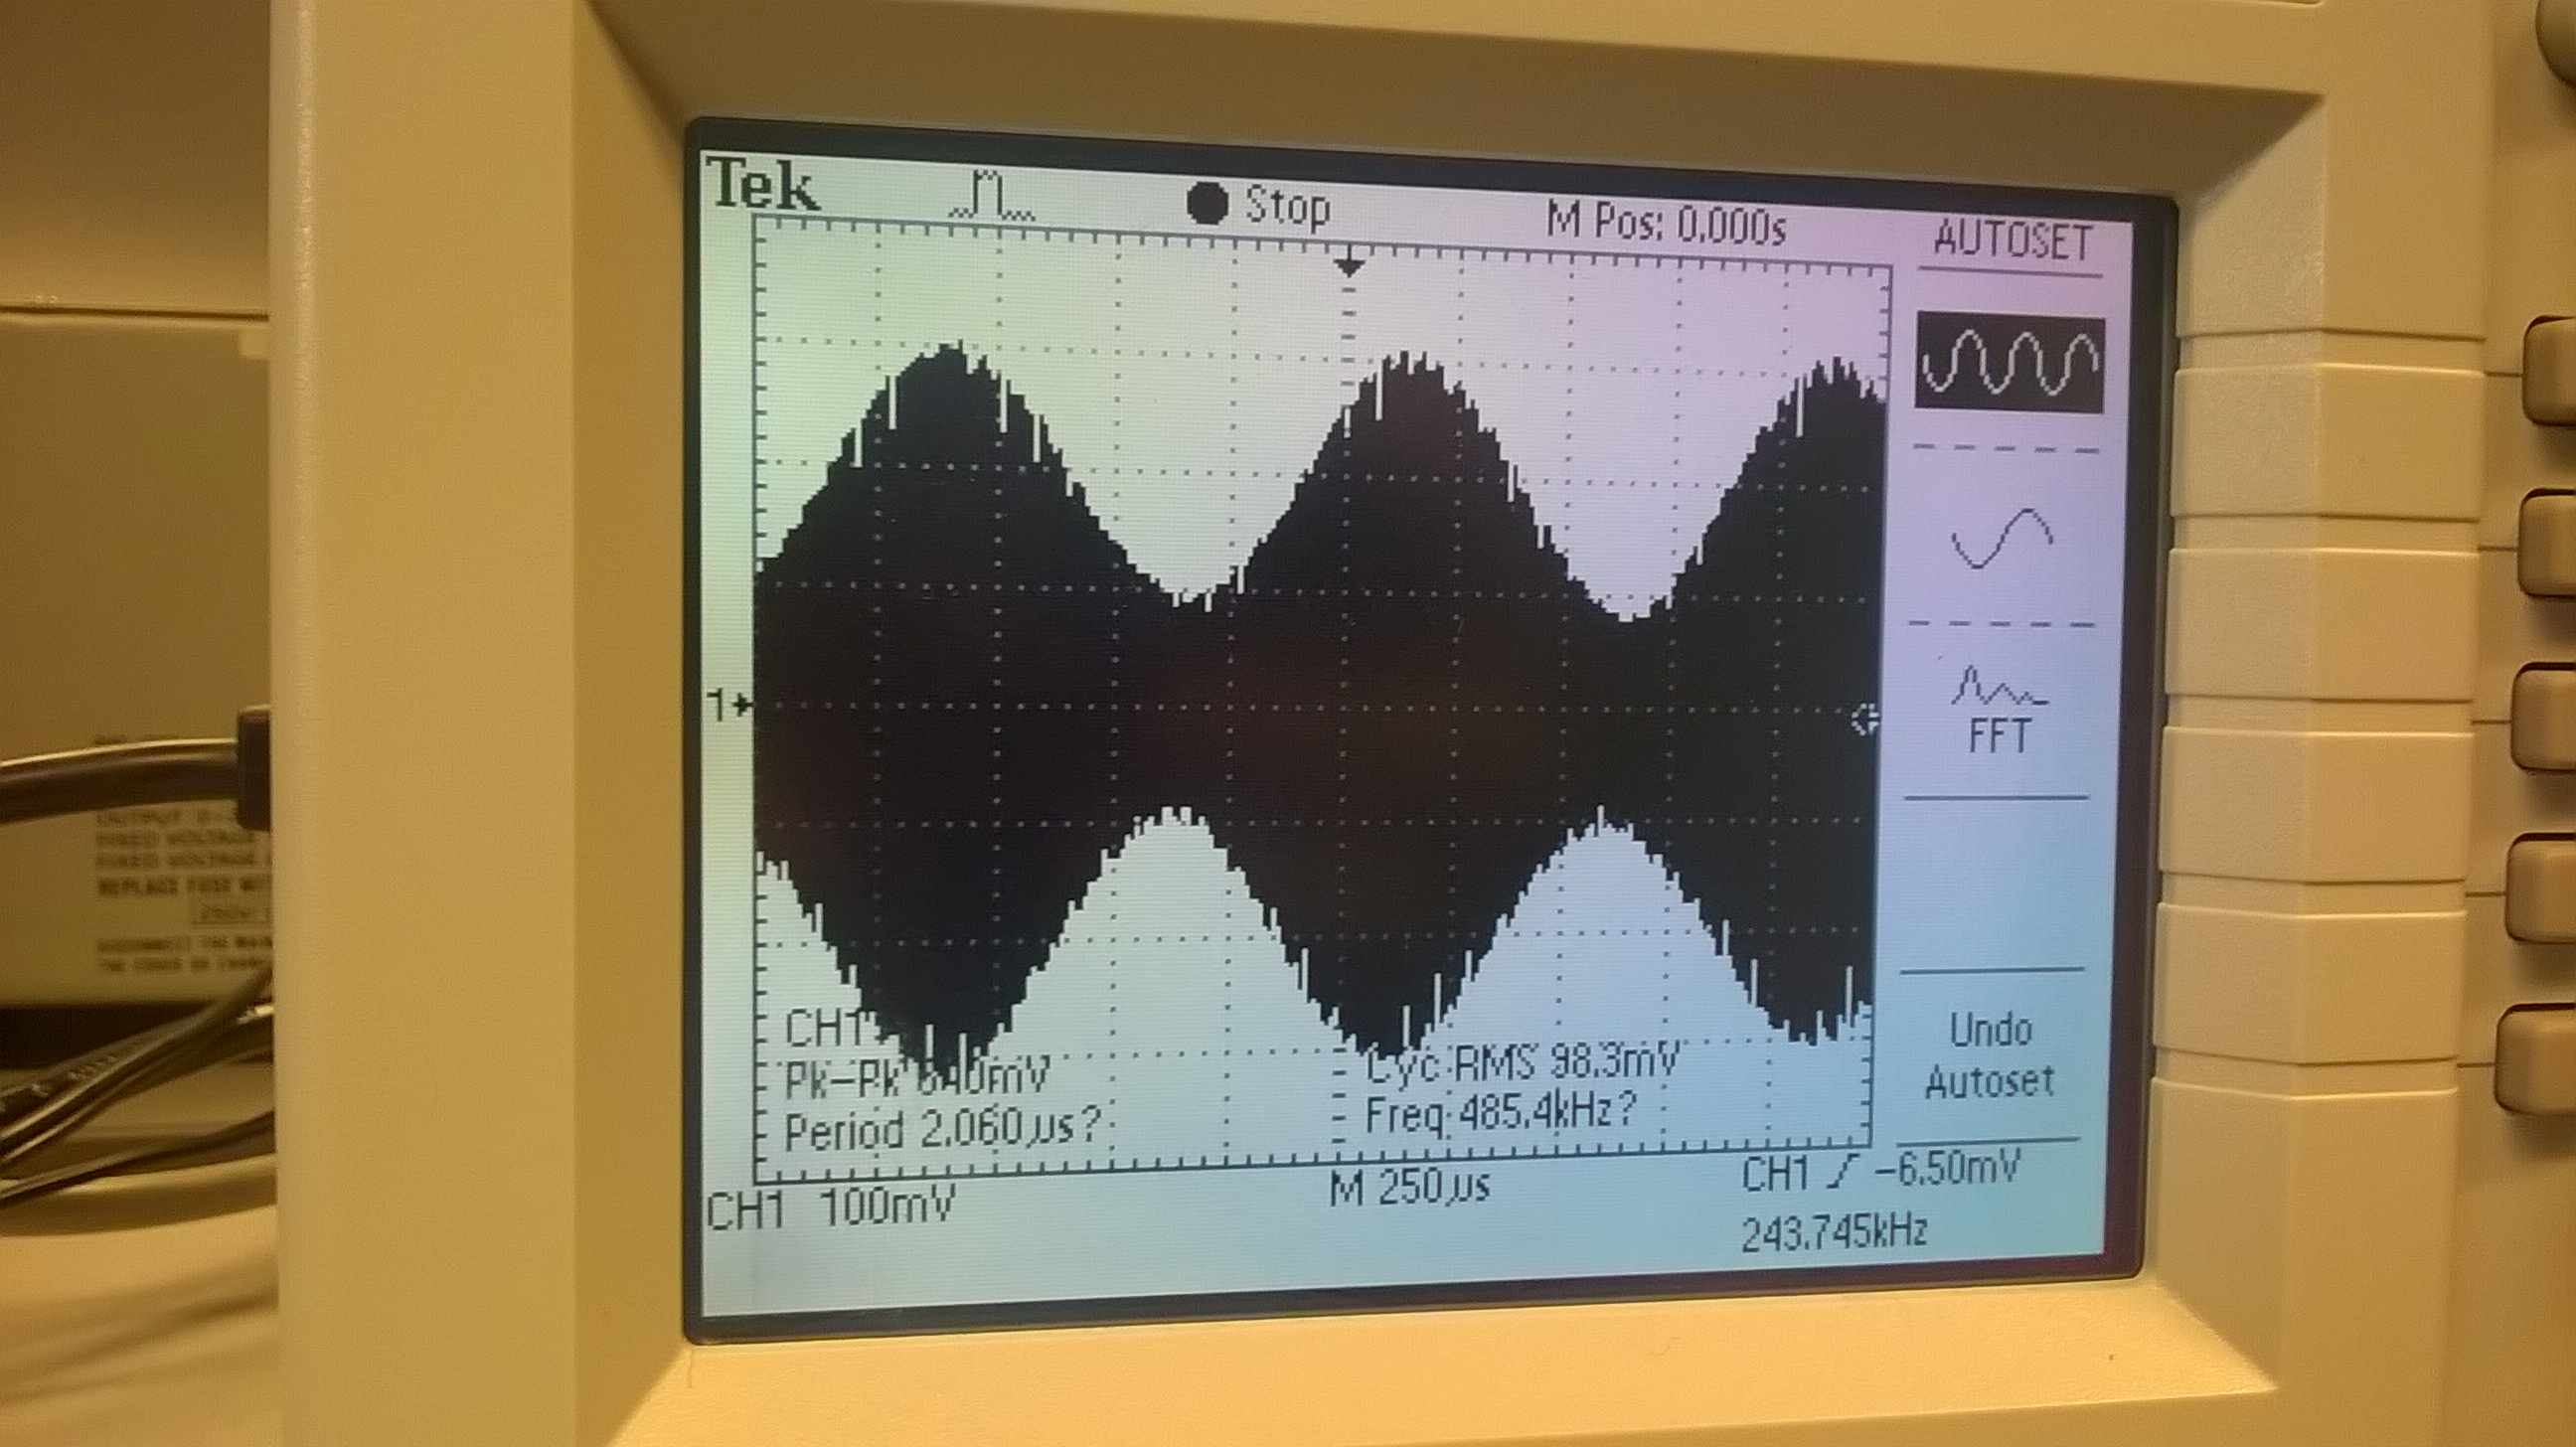
\includegraphics[scale=0.1]{AM/4Modul2}}
\caption{The modulated signal output}
\end{figure}
The signal was too complicated for our oscilloscope to make FFT analysing. That's why we used spectrum analyser to measure it, the device also has cursors which helped us to make more accurate measurements. In our sine-wave difference between main peak the second\footnote{biggest beside other} ones\footnote{there are two peaks with approximately same altitude on negative and positive sides} should be about 800Hz, and it can help us to check the quality of our modulation.
\begin{figure}[H]
\centerline{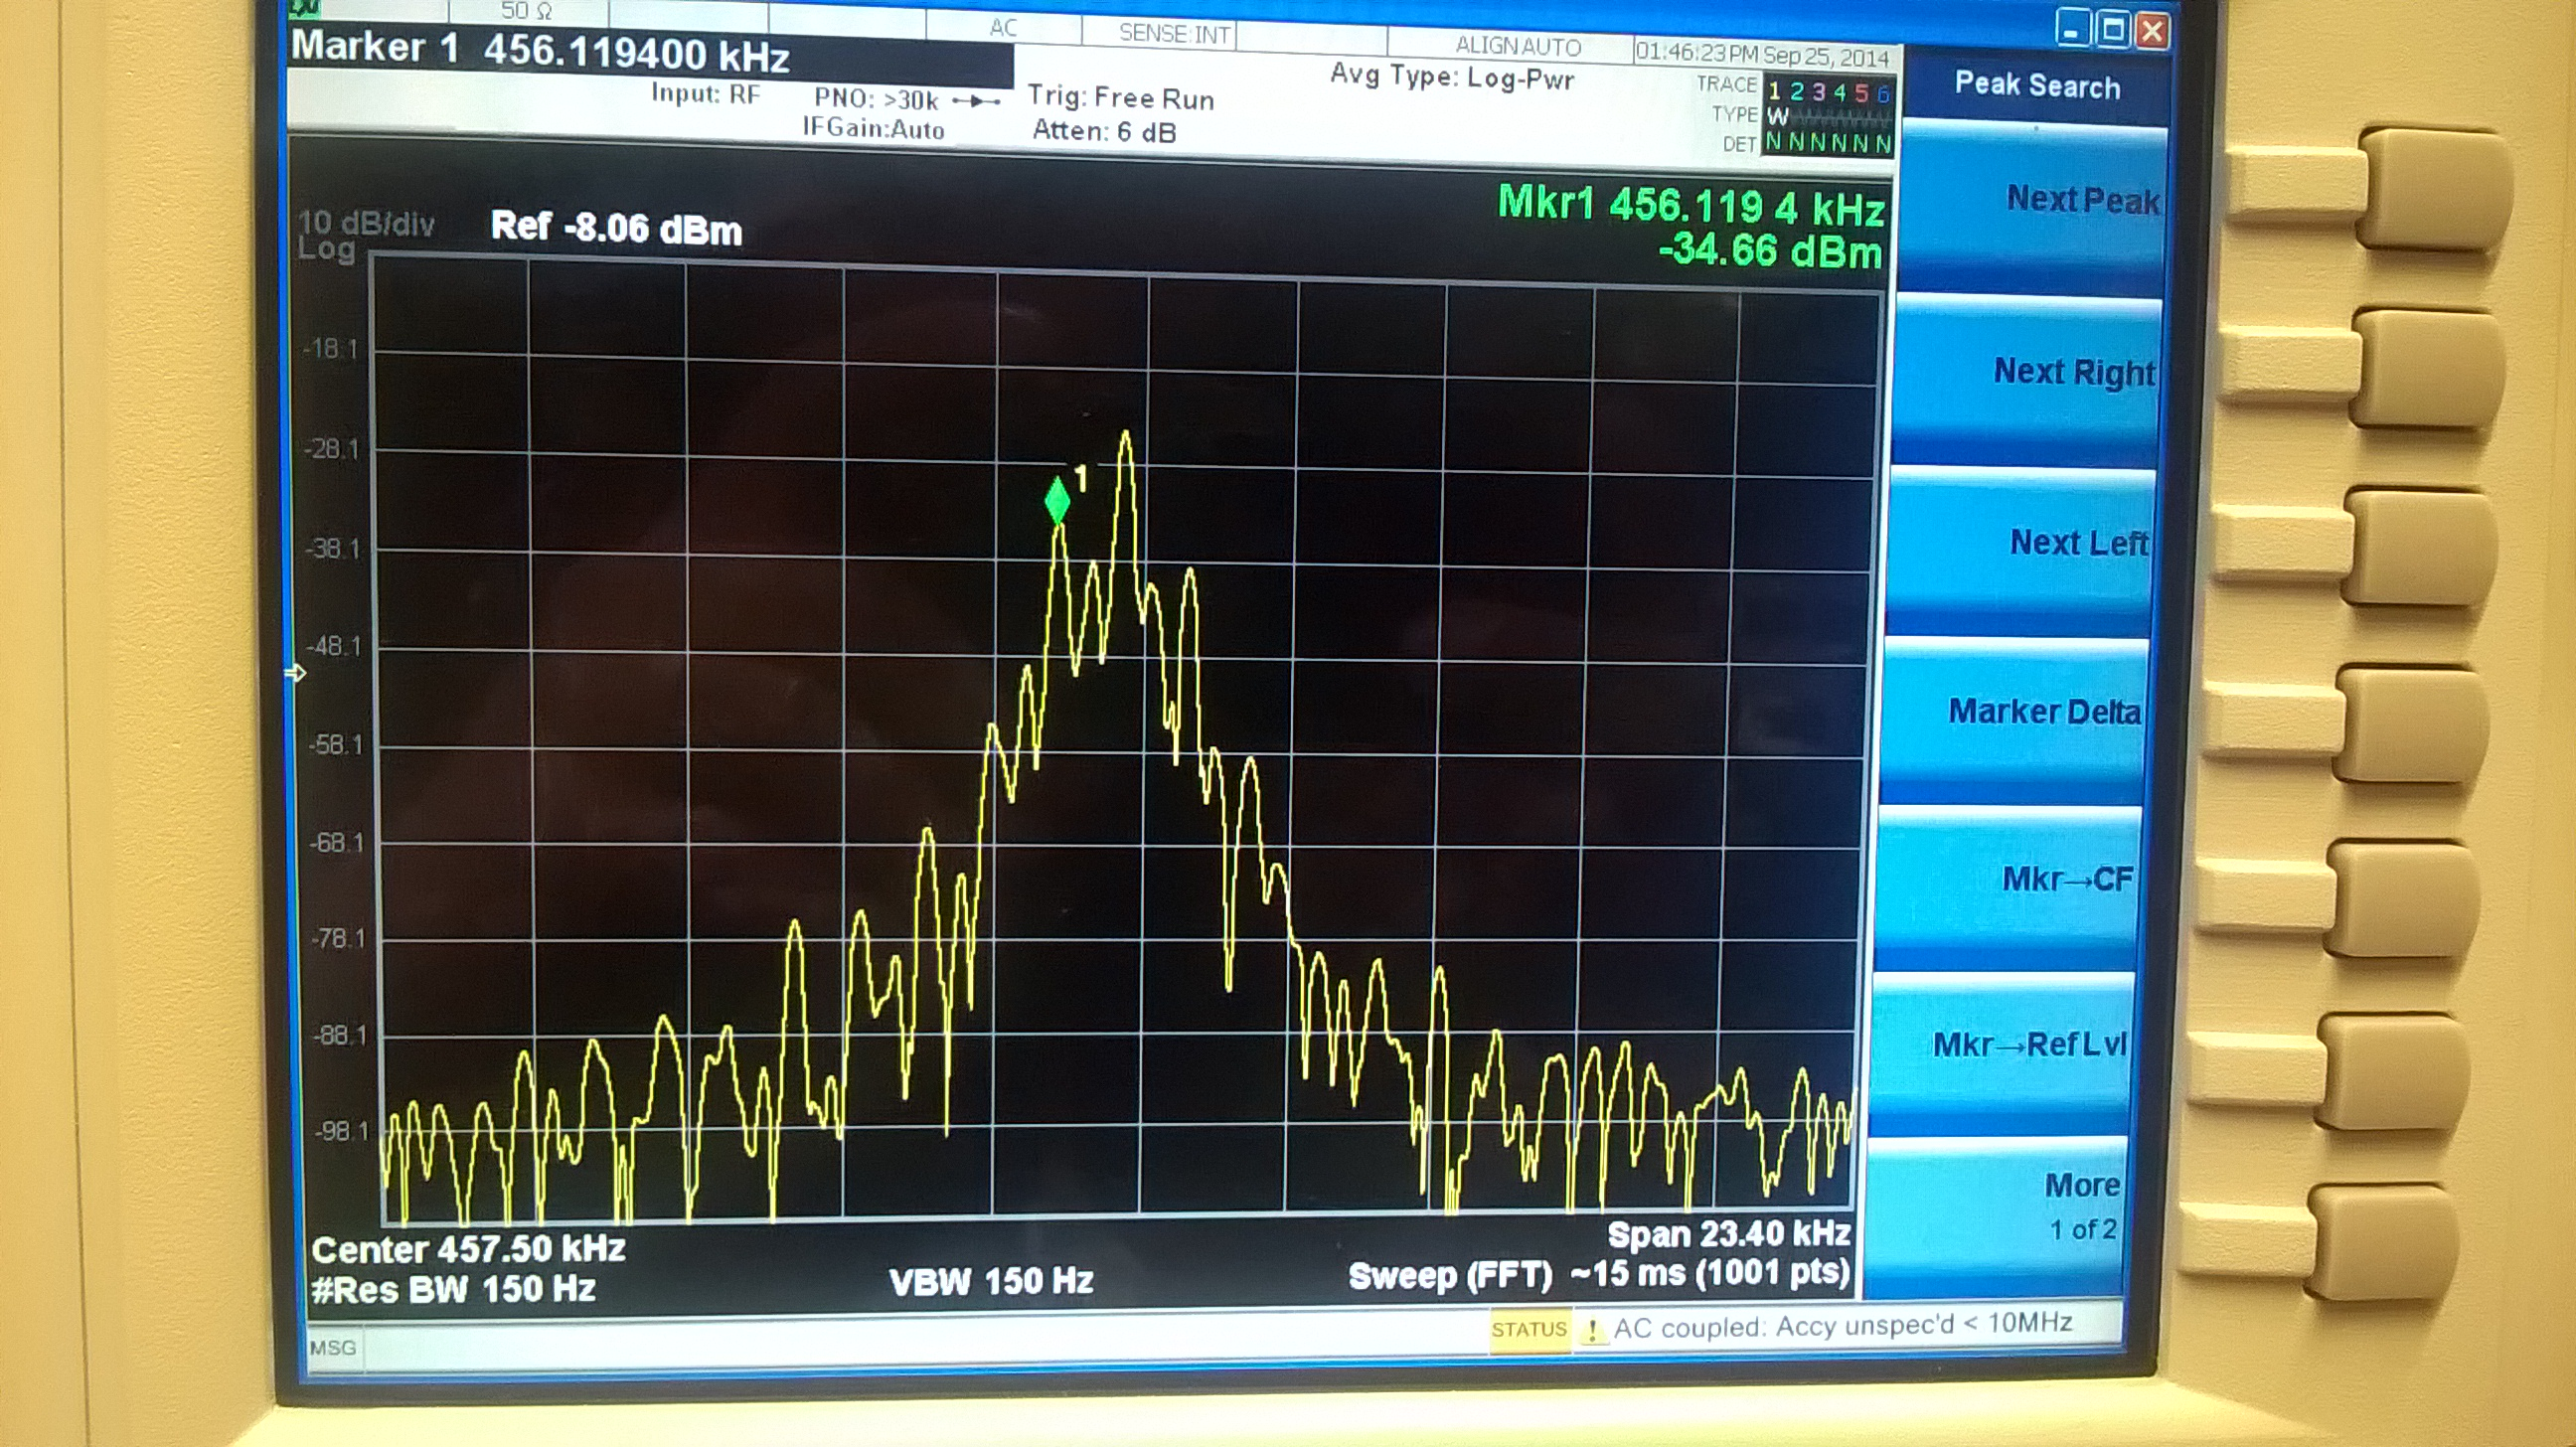
\includegraphics[scale=0.1]{AM/WP_20140925_021}}
\caption{The modulated signal FFT, measurement of the negative small peak deviation}
\end{figure}
The central peak has 457.145kHz, the left one is 458.155kHz and the right equals 456.119kHz. Let us calculate $\Delta f_L$ and $\Delta f_R$.
$$
\Delta f_L=457.145kHz-456.119kHz=1026Hz
$$
$$
\Delta f_R=458.155kHz-457.145kHz=1010Hz
$$
\begin{figure}[H]
\centerline{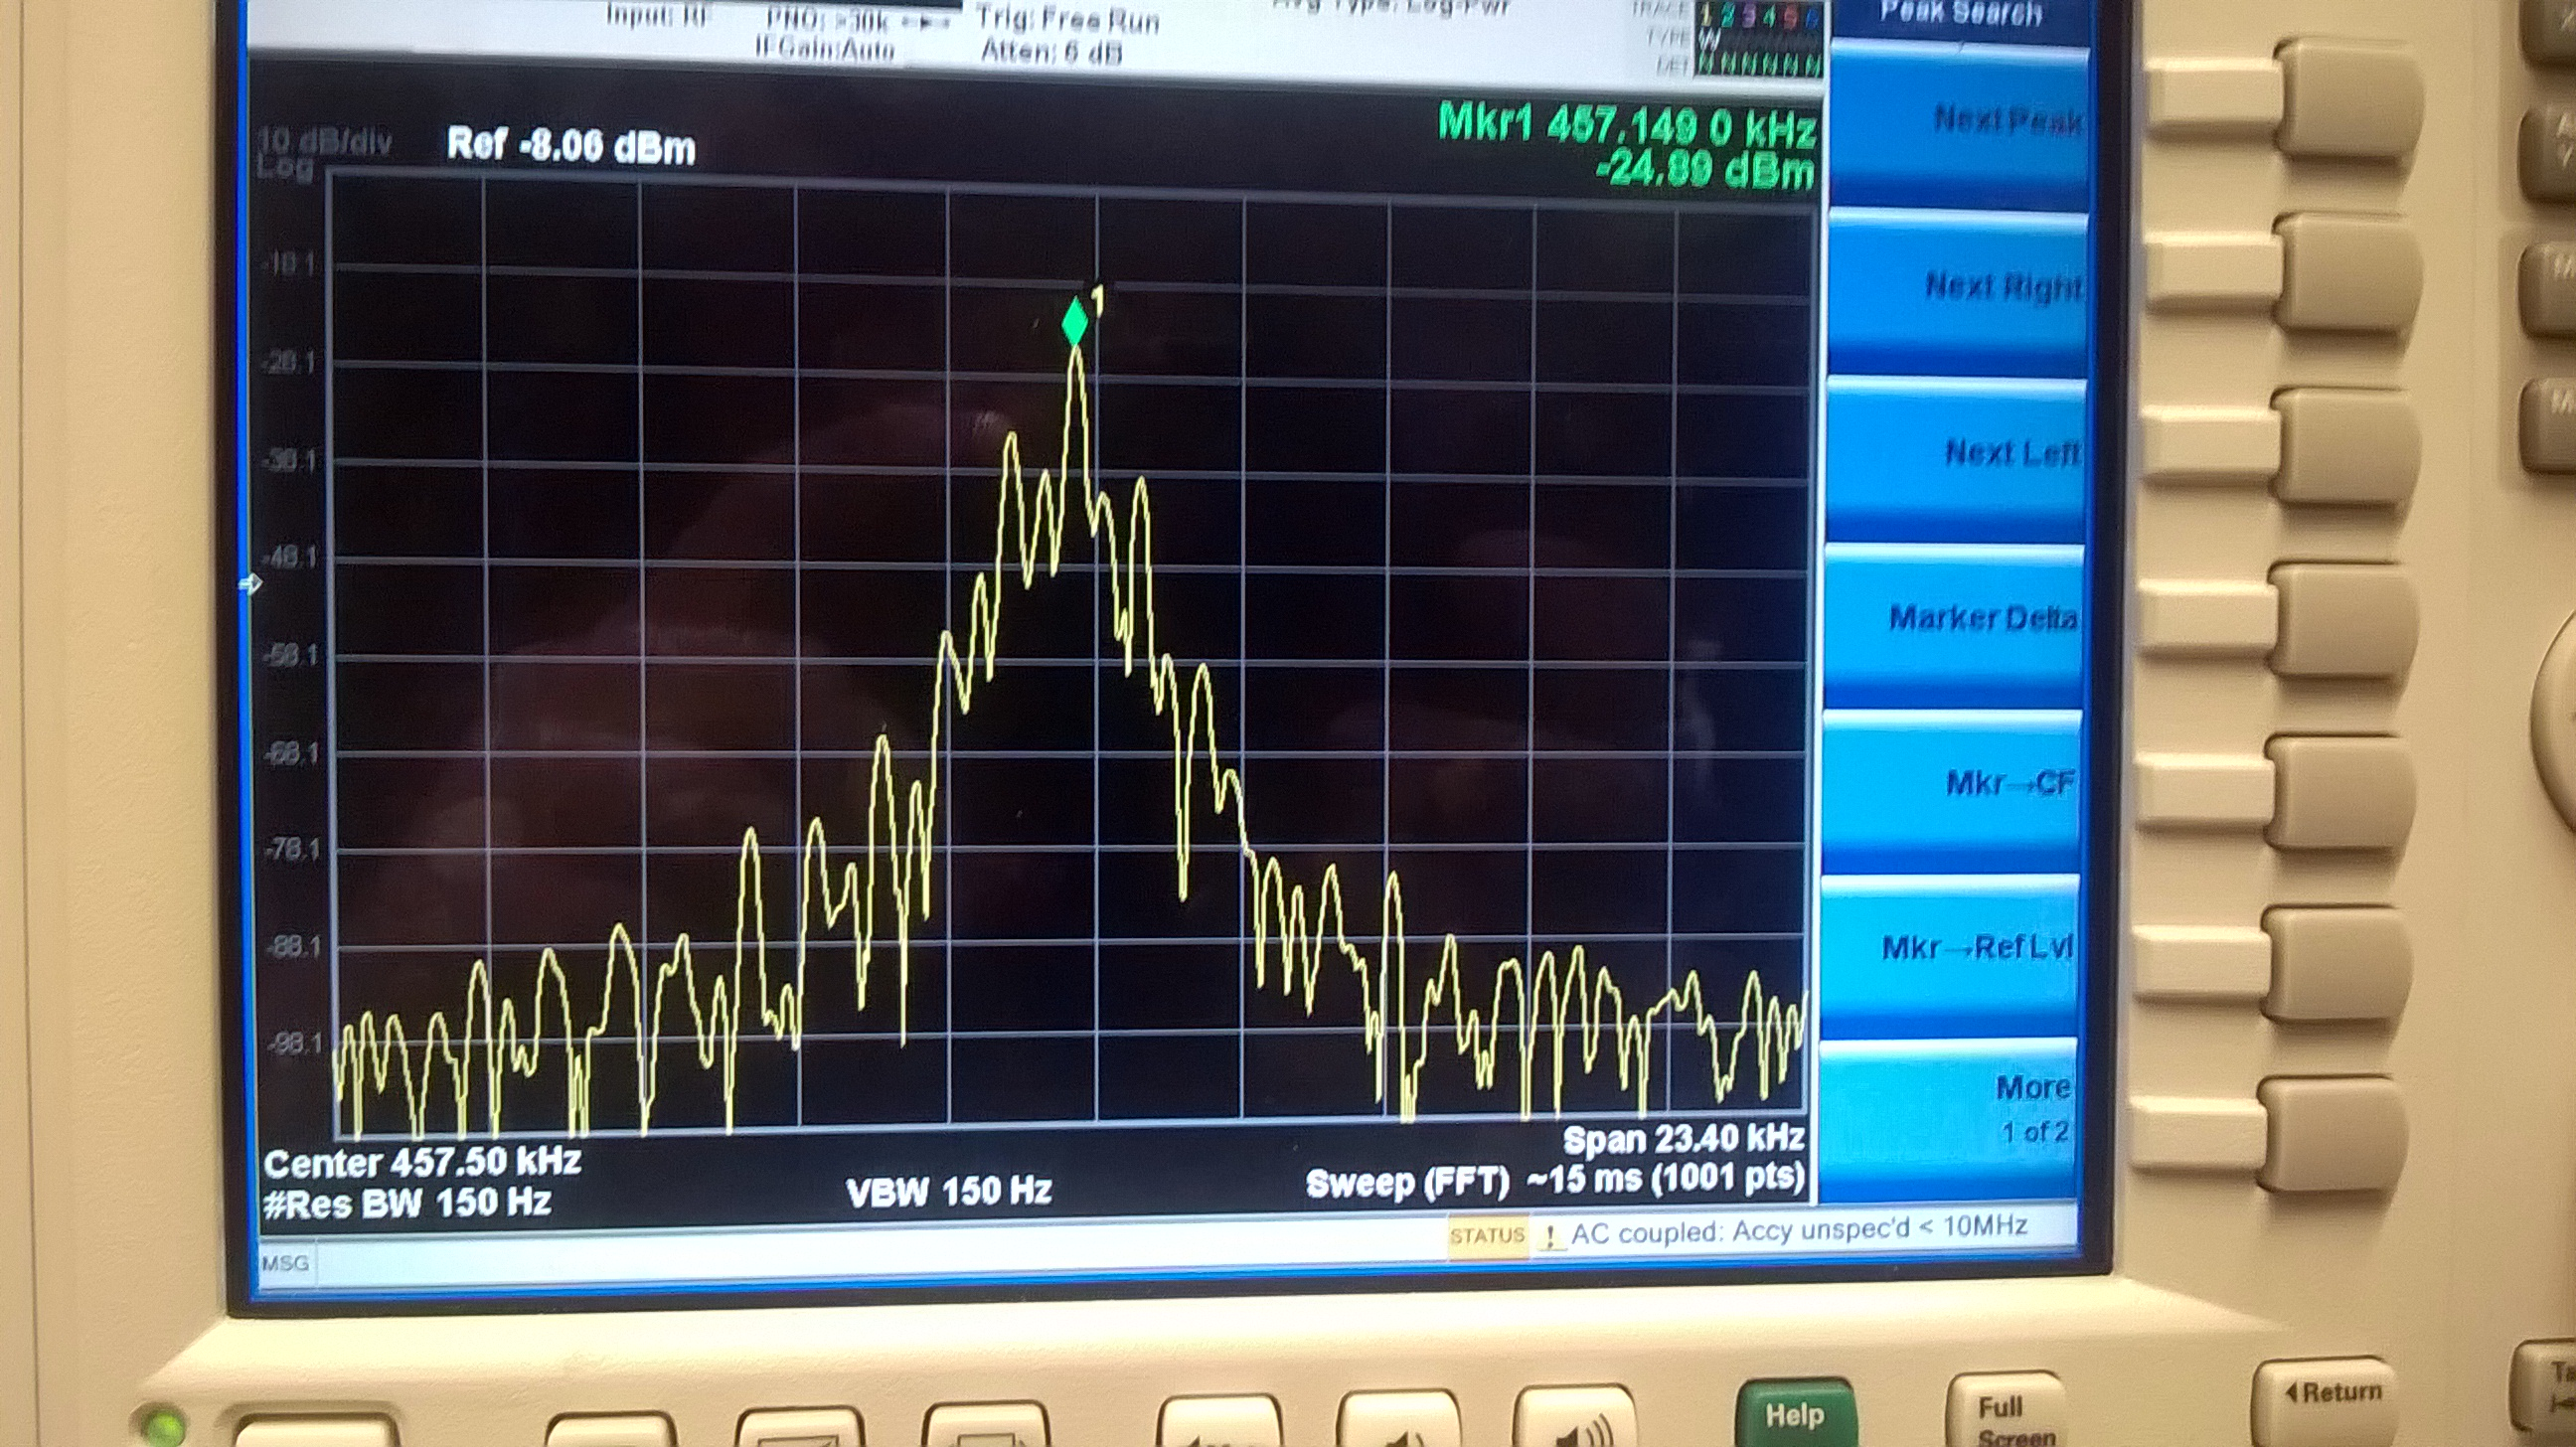
\includegraphics[scale=0.09]{AM/WP_20140925_022}}
\caption{The modulated signal FFT, measurement of the central peak}
\end{figure}
\begin{figure}[H]
\centerline{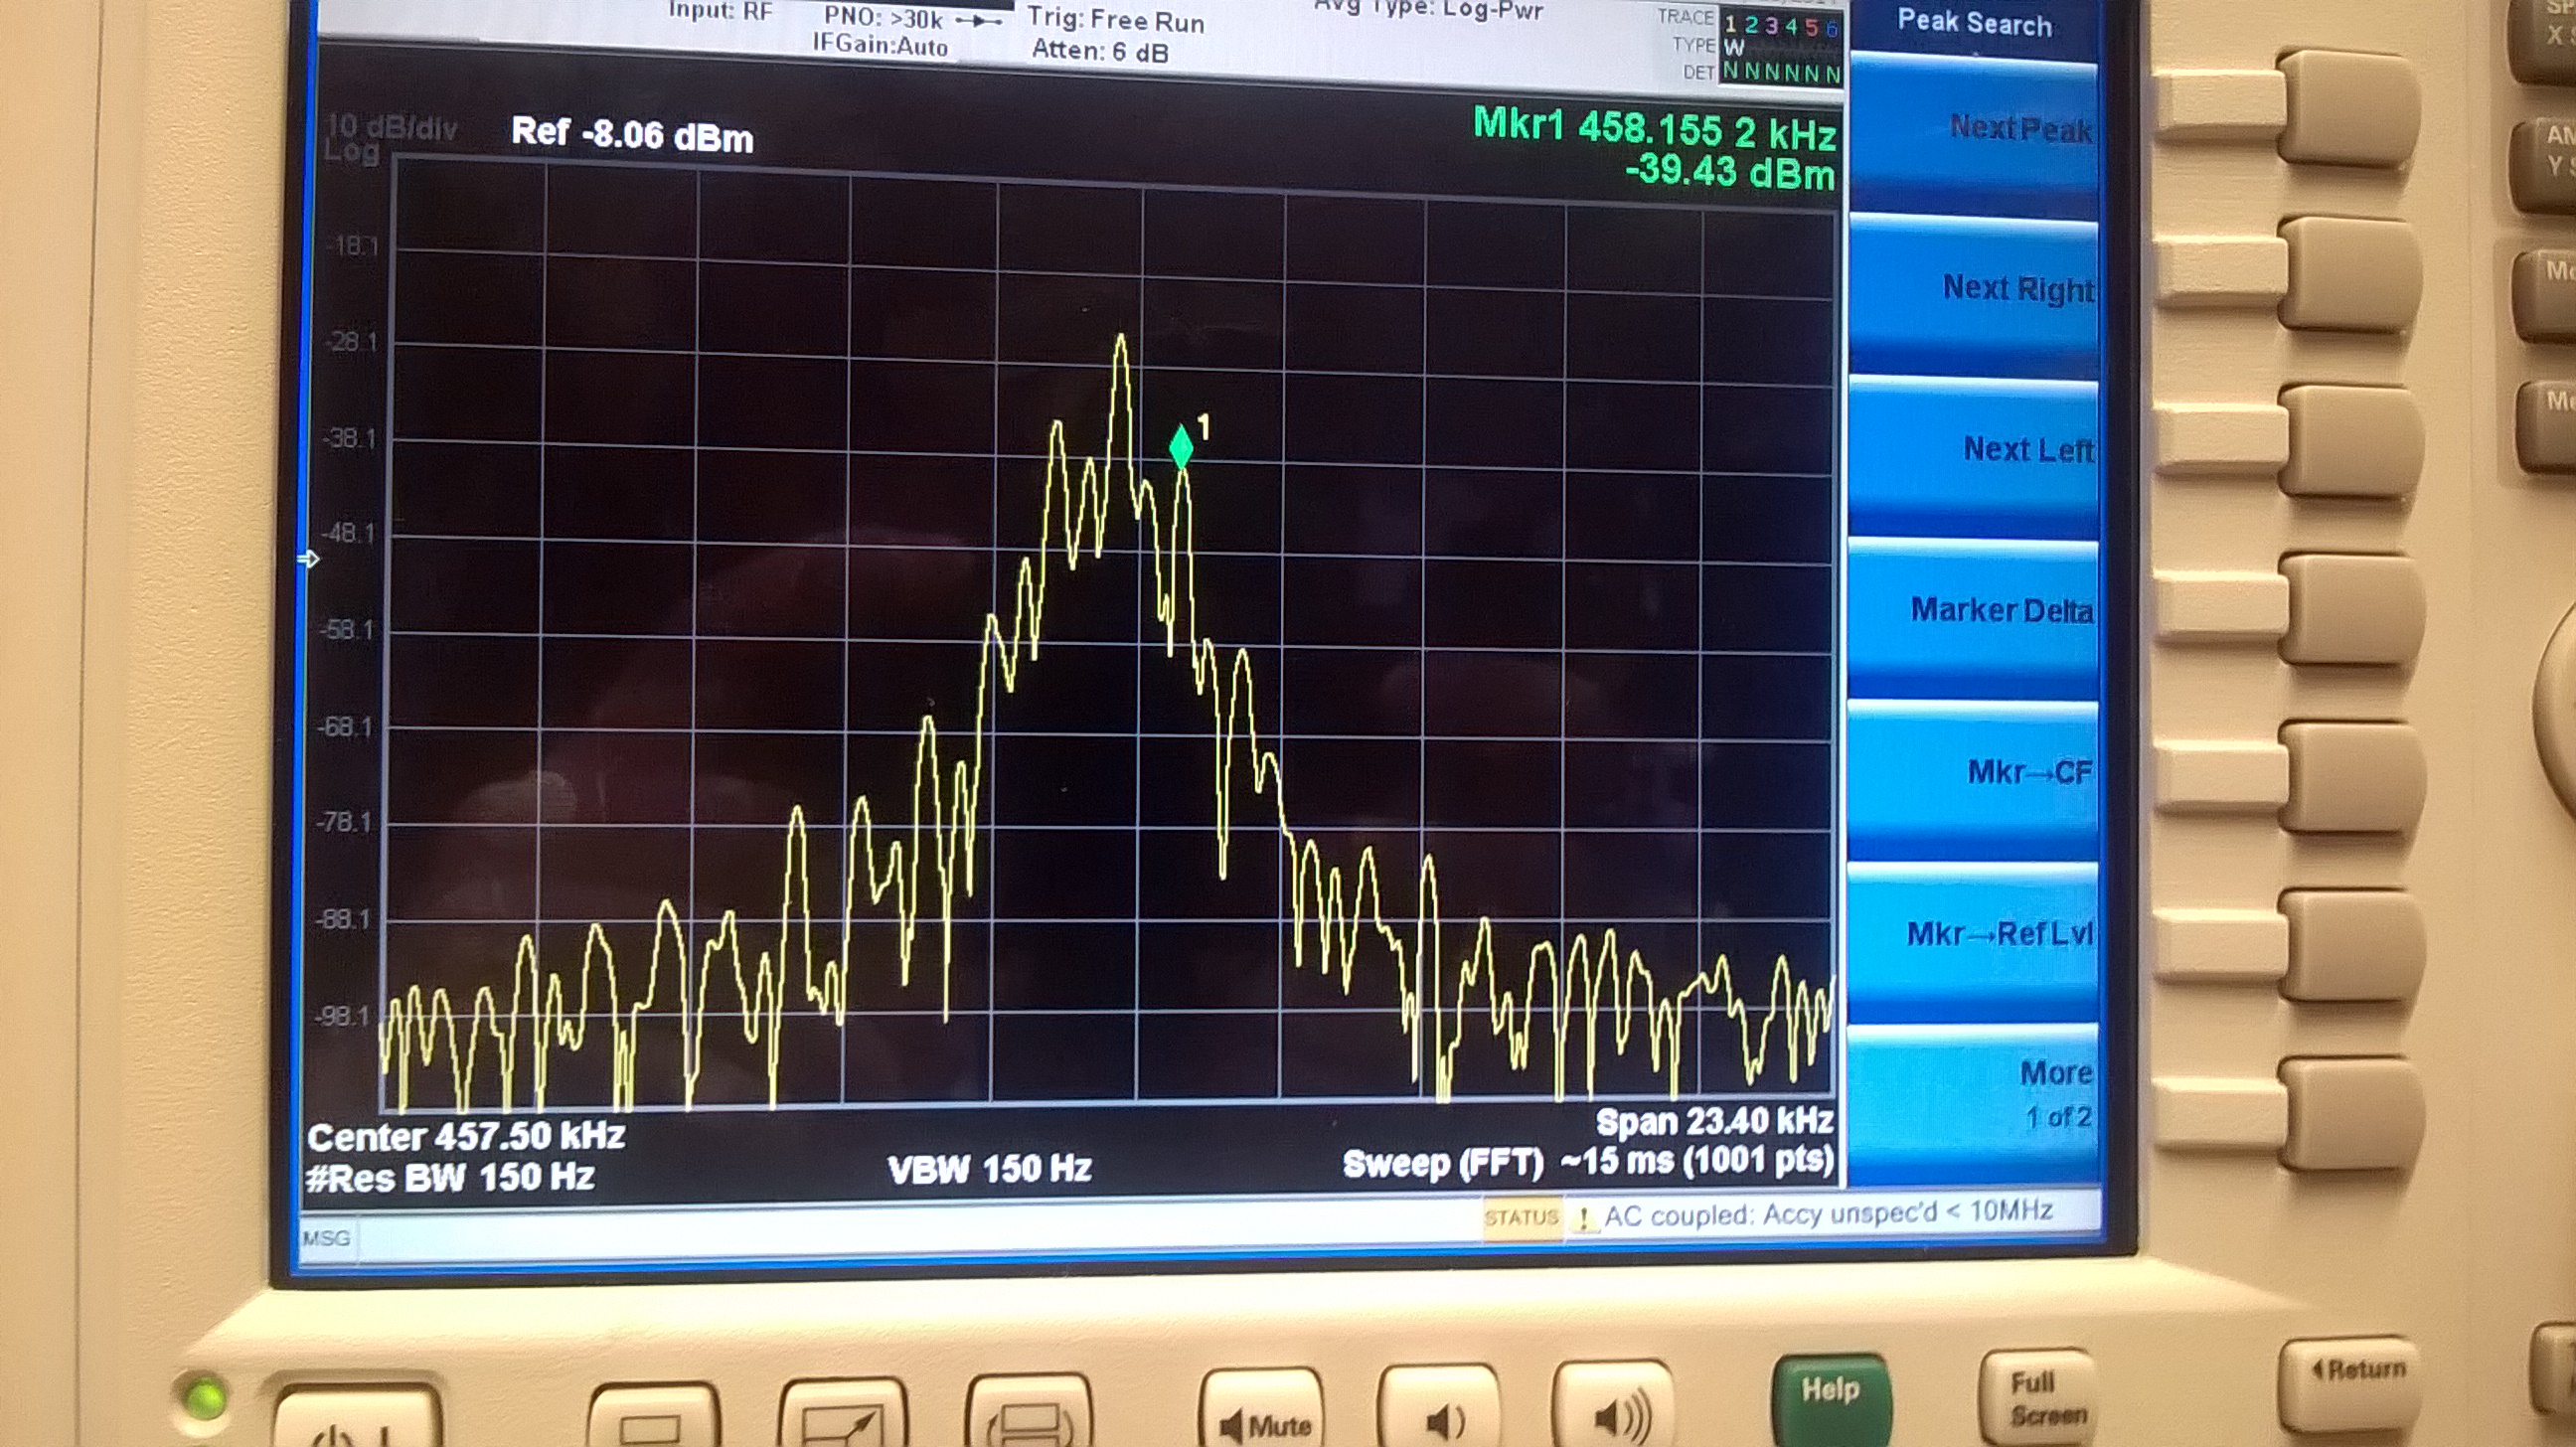
\includegraphics[scale=0.09]{AM/WP_20140925_023}}
\caption{The modulated signal FFT, measurement of the positive small peak deviation}
\end{figure}
\subsubsection{Result}
The modulation was made successfully, $\Delta f_L$ and $\Delta f_R$ are very close to desirable result, the difference is result of the fact that the measurement was made on the signal which modulation was not full, the signal was modulated approximately by 50\%, but it was enough to study the process of modulation in a piratical exercise.

\subsection{Demodulation}
We used product detector to demodulate our signal. The method is the most modern one and it contains two steps.
The IF and its FFT are demonstrated on the figures 10 and 11.
\begin{figure}[H]
\centerline{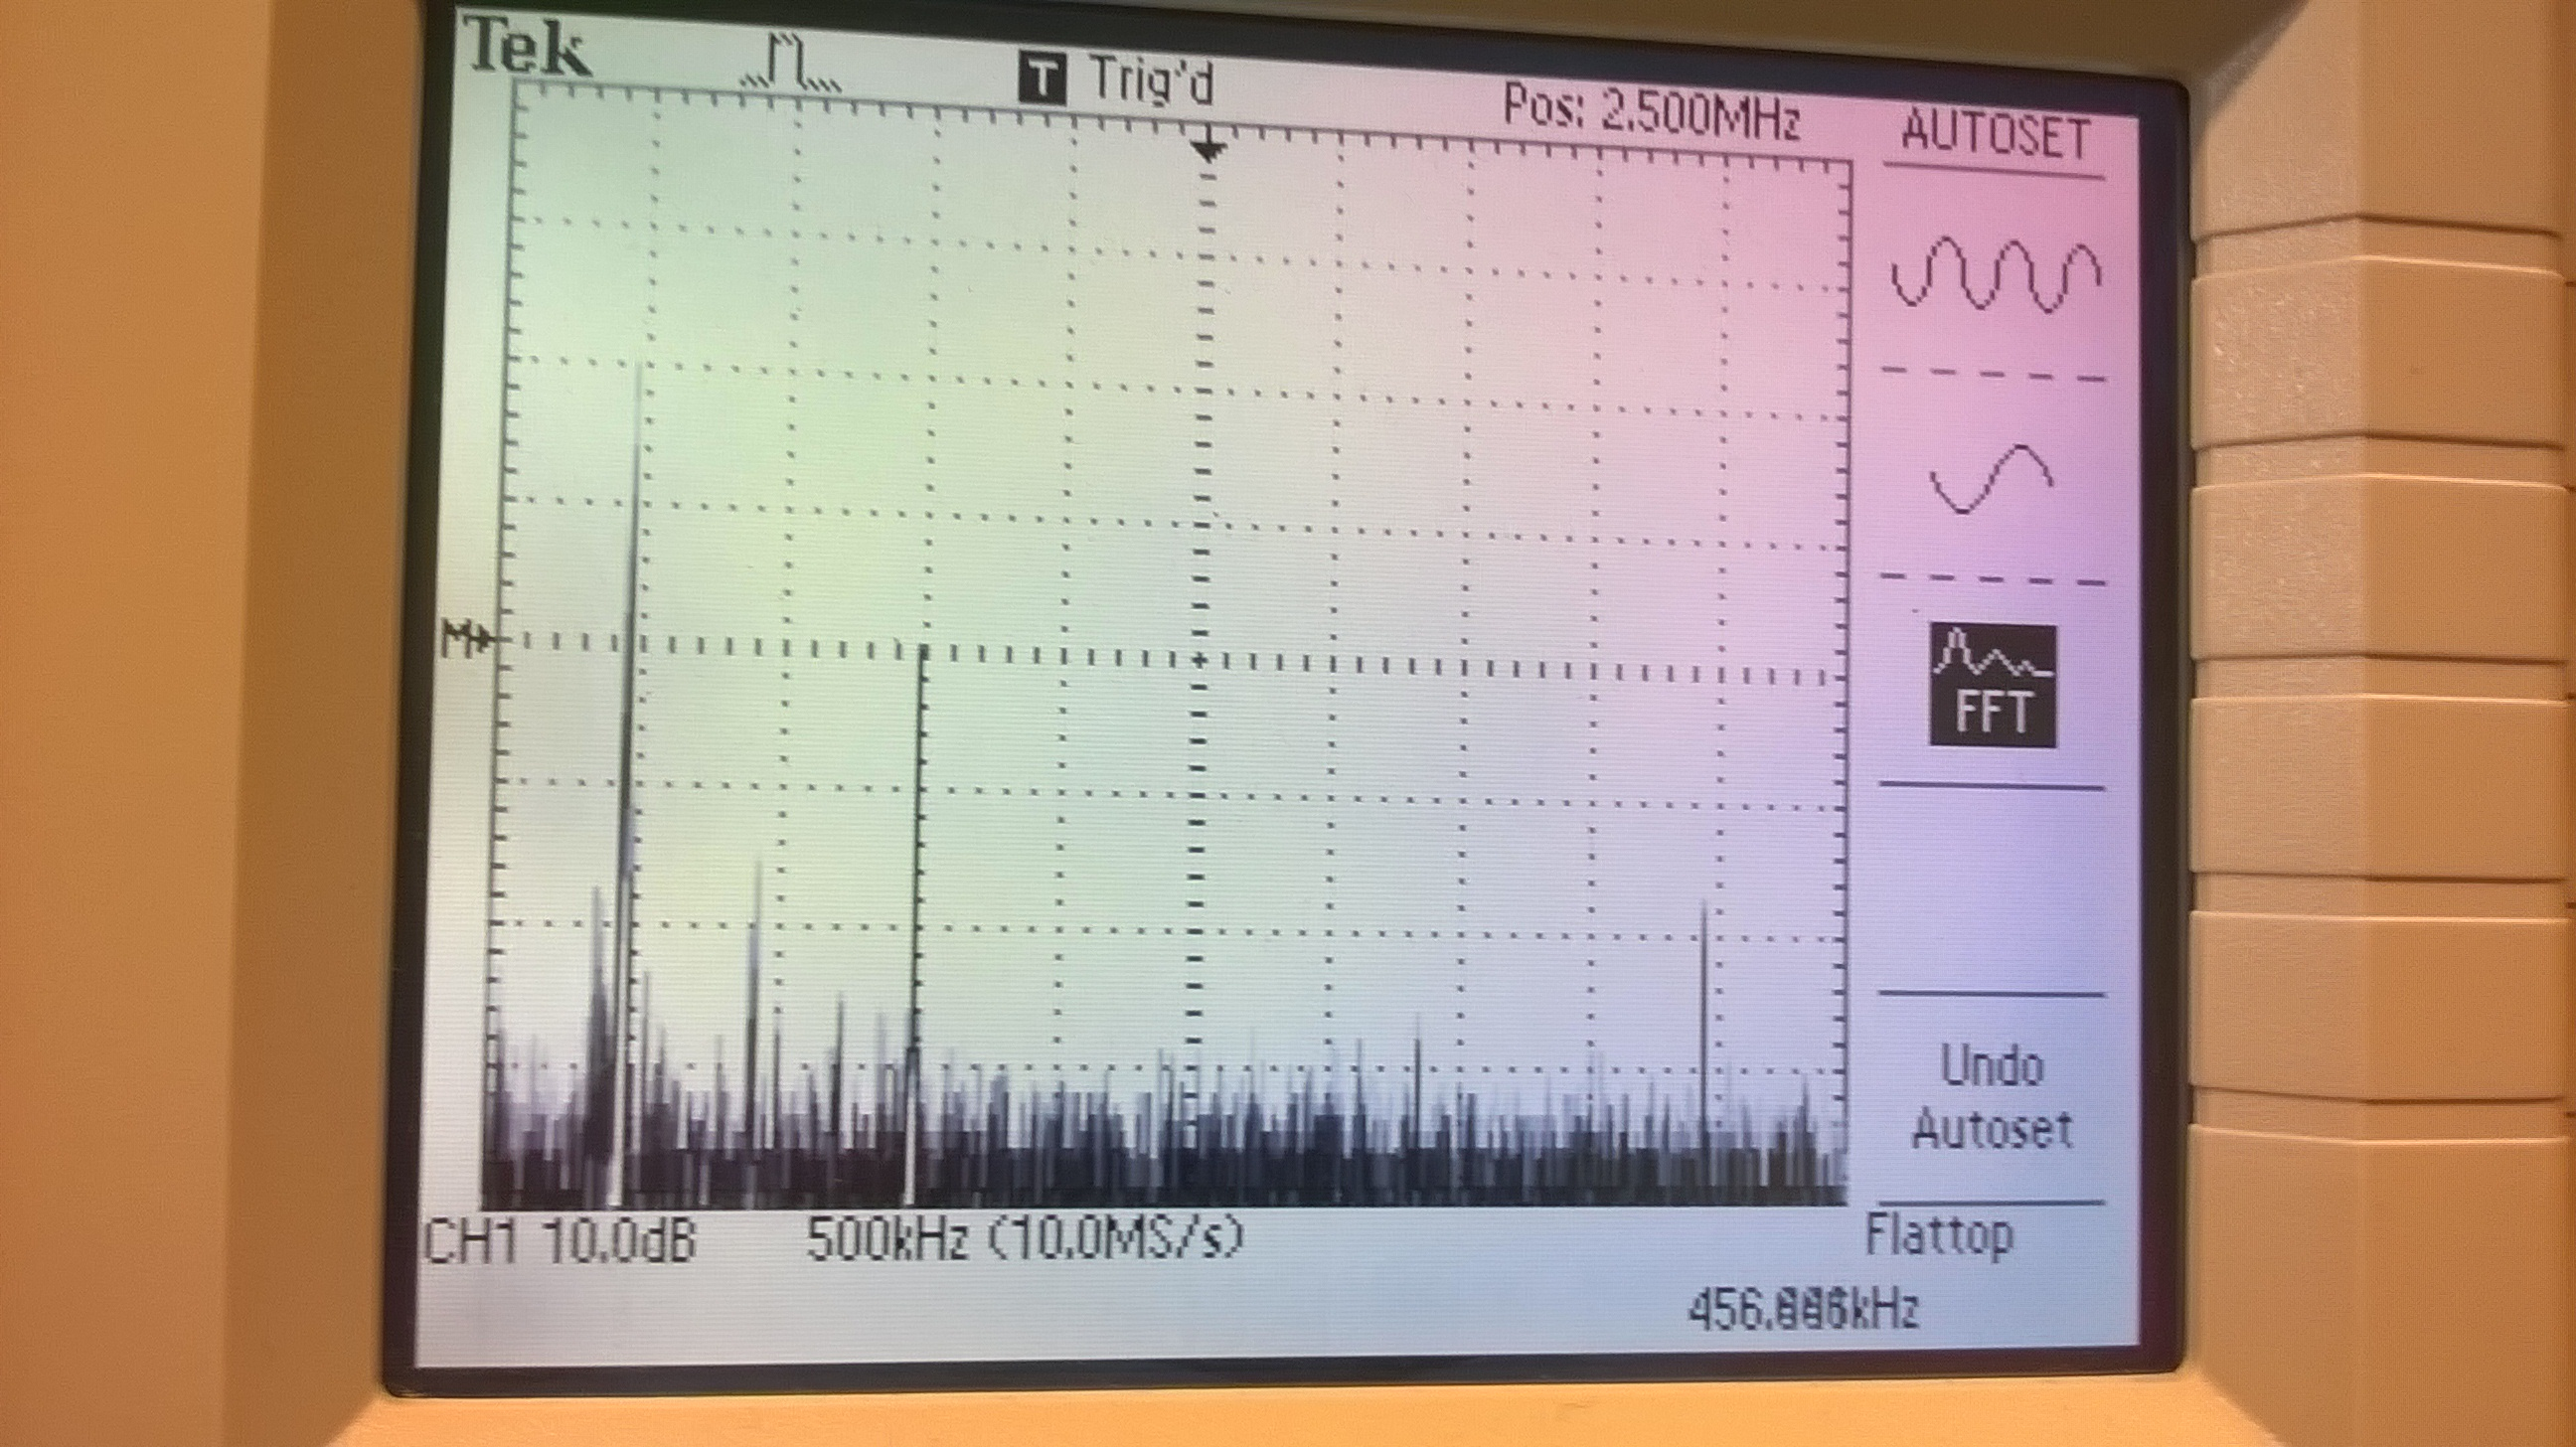
\includegraphics[scale=0.09]{AM/8_IF1}}
\caption{IF FFT}
\end{figure}
At the first step the signal should be mixed with high frequency local oscillator's wave, to move our signal to intermediate frequency(IF), after that the IF would be filtered to detect the initial signal. \\\\

\begin{figure}[H]
\centerline{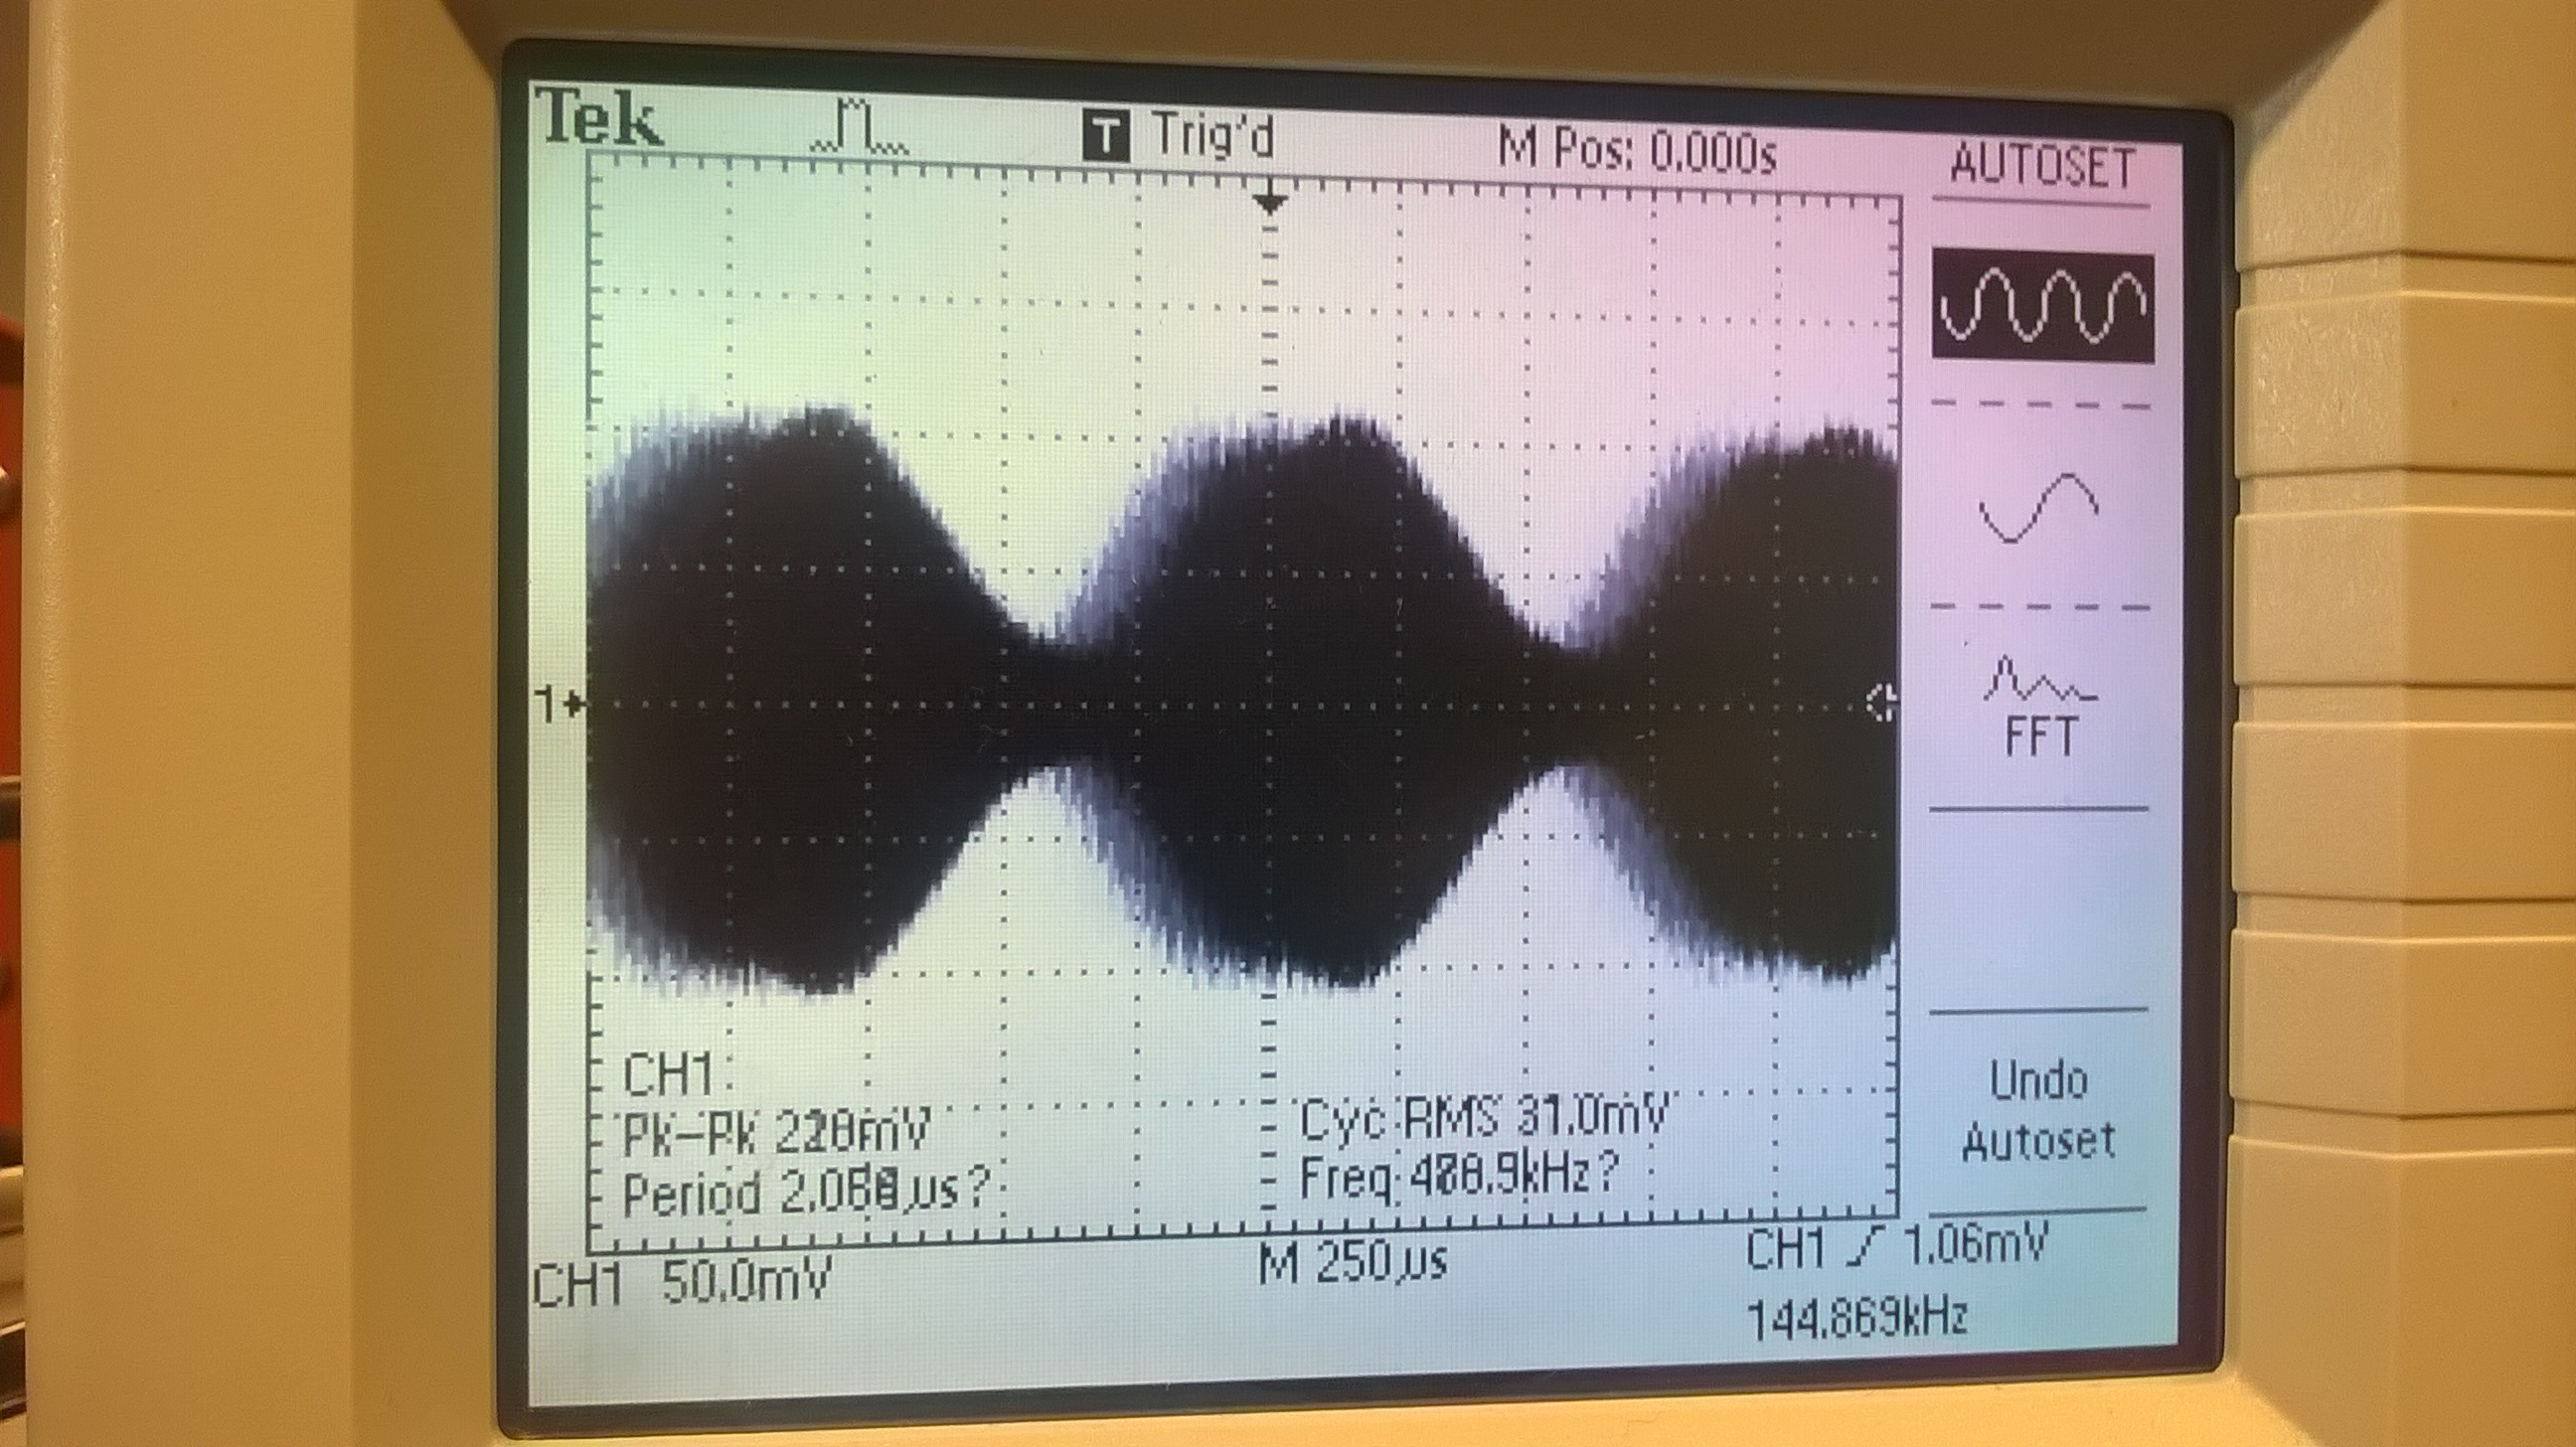
\includegraphics[scale=0.1]{AM/9_IF2}}
\caption{IF signal}
\end{figure}
\subsubsection{Result}
The final output is demonstrated on the picture 12. You can see that the signal doesn't have a sin wave form, but the frequency is correct and information is transmitted well.
\begin{figure}[H]
\centerline{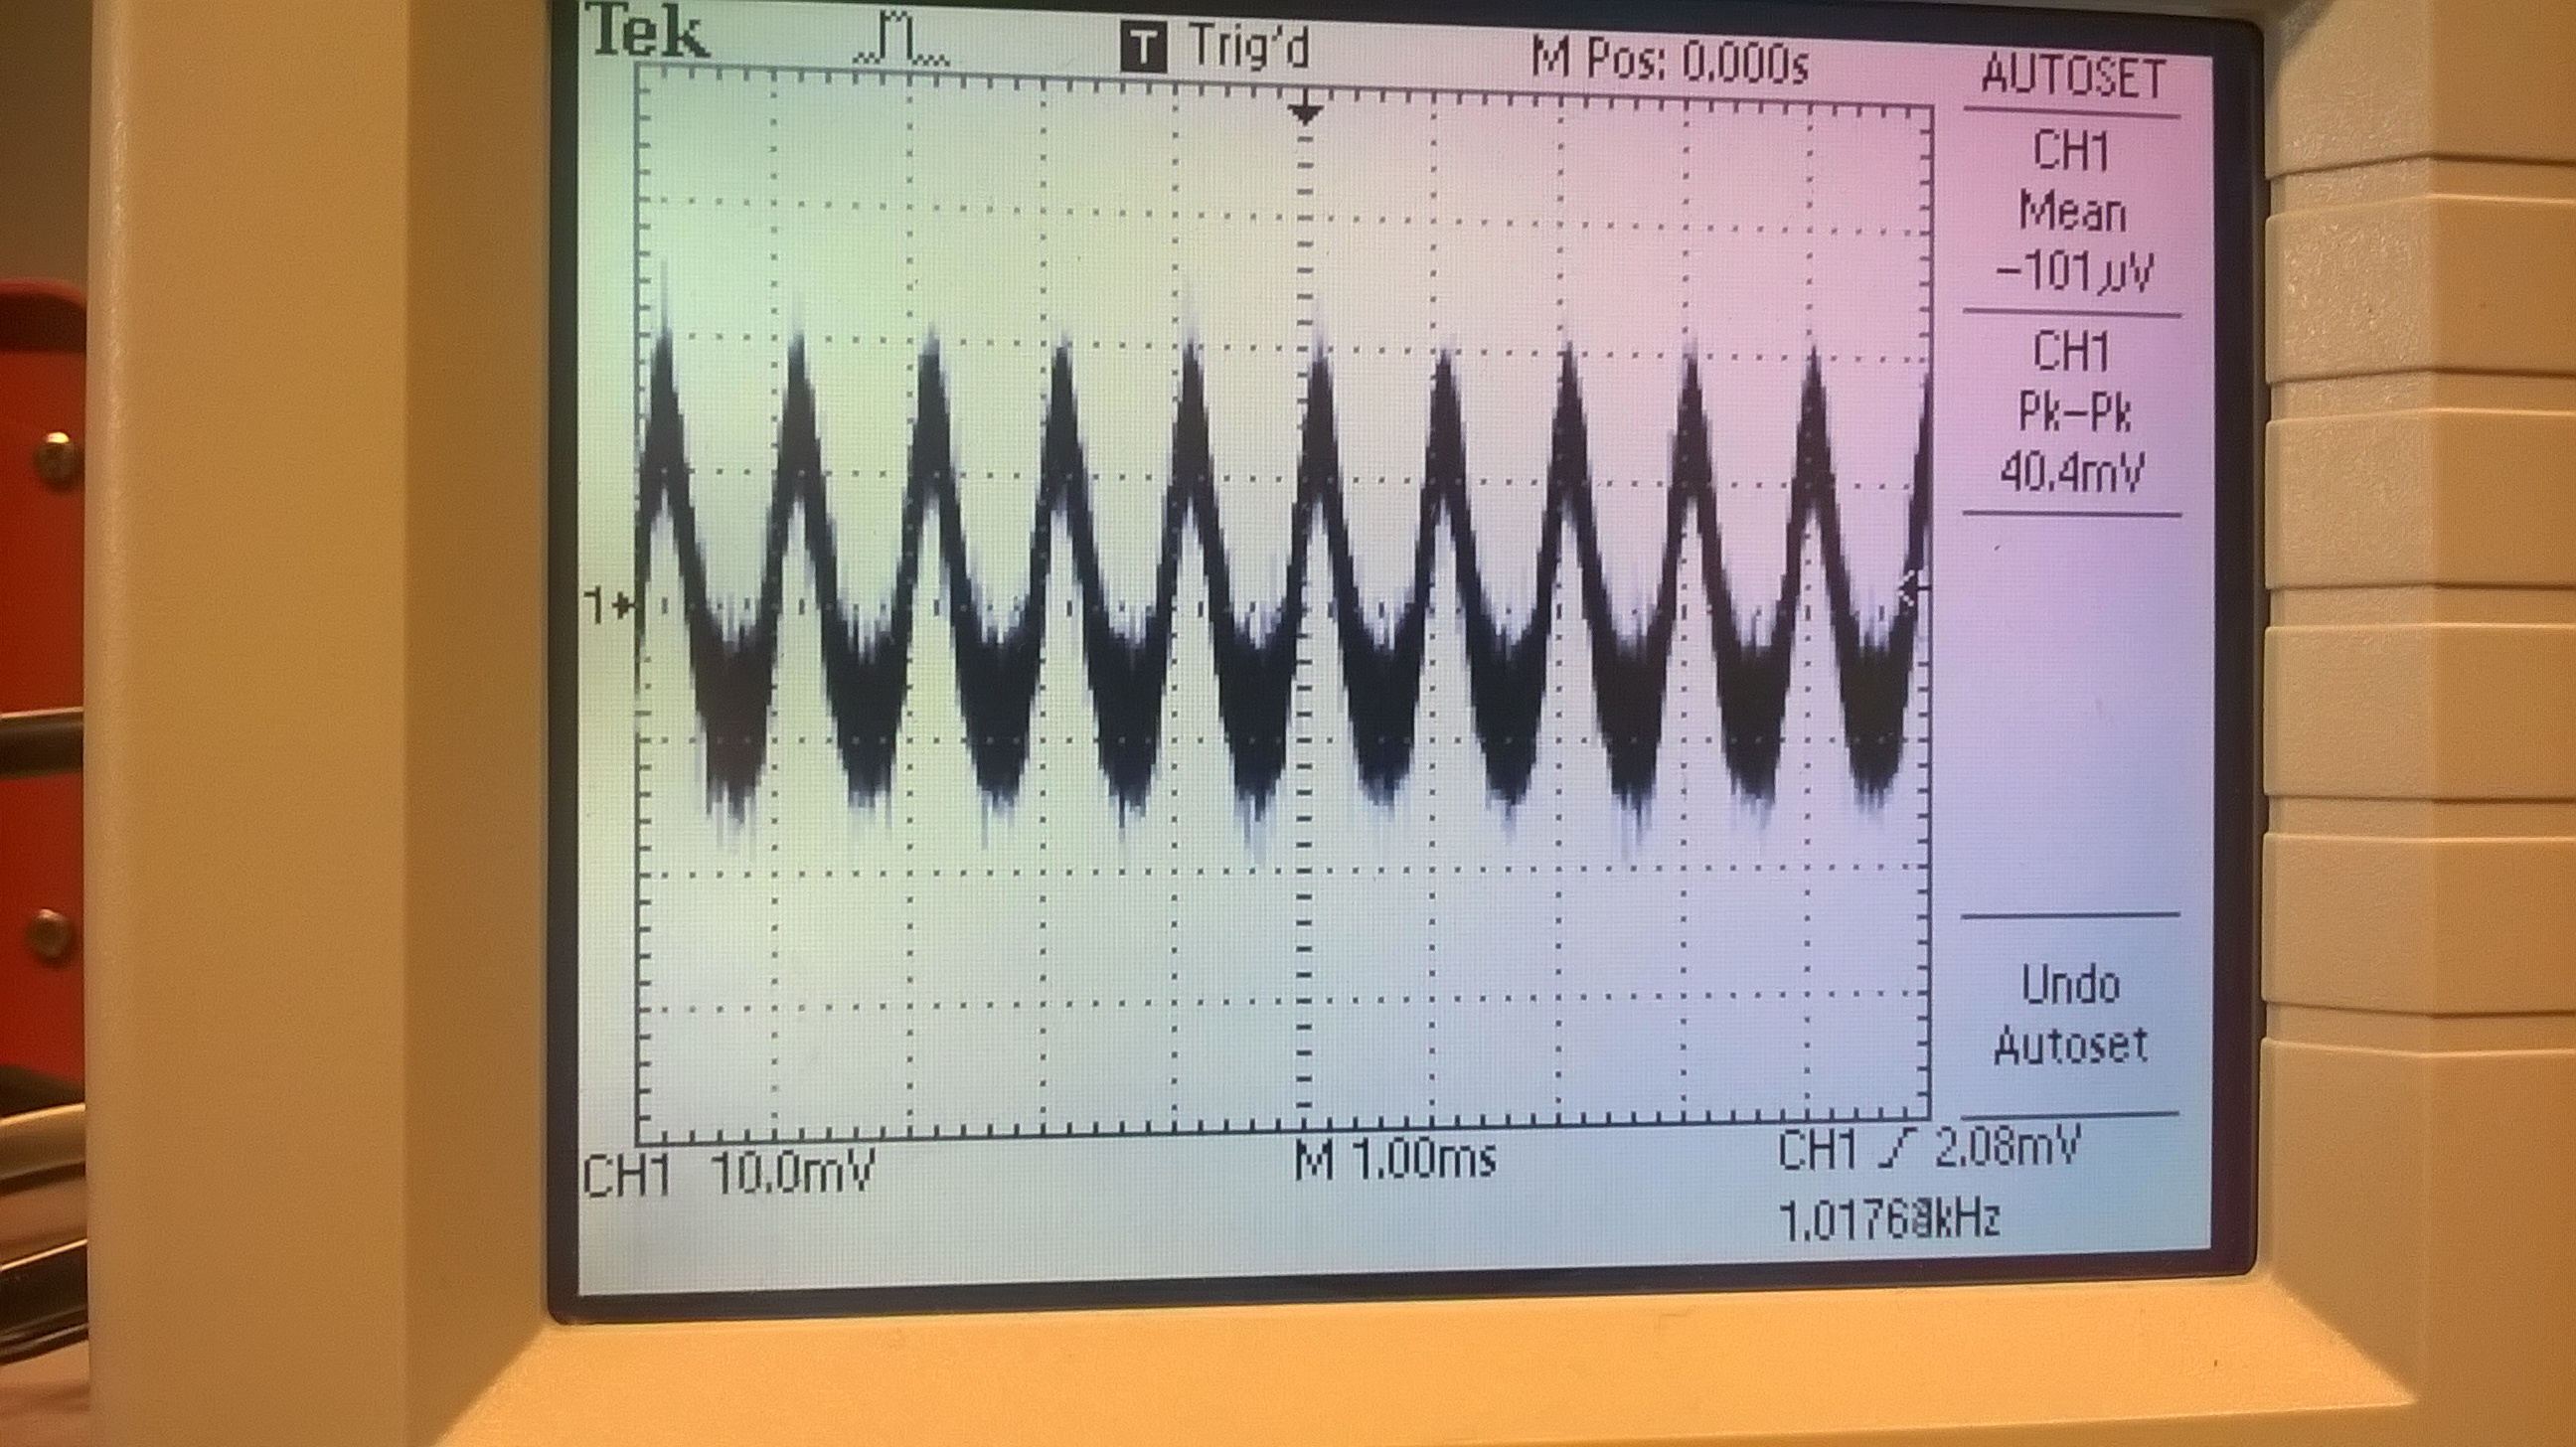
\includegraphics[scale=0.1]{AM/12Result}}
\caption{IF signal}
\end{figure}
\section{Conclusion}
During the lab work we have successfully modulated and demodulated low-frequency signal by AM, we studied the modulation/demodulation process on a practice, make our understanding deeper and became familiar with the wave forms and transformations in the Amplitude Modulation.



\end{document}
